\documentclass[11pt,a4paper]{article}
\usepackage[a4paper]{geometry}
\usepackage{cite}
\usepackage{graphicx}
\usepackage{epsfig,rotating}
\usepackage{amssymb}
\usepackage{mathrsfs}
\usepackage{amsmath}
\usepackage{amsfonts}
\usepackage{multirow}
\usepackage{eurosym}
\usepackage{dcolumn}
\usepackage{microtype}
\usepackage{multirow}
\usepackage{enumitem}
\usepackage{booktabs}
\usepackage{bm}
\usepackage{dcolumn}
\usepackage[hyphens]{url}
\usepackage{hyperref}
\usepackage{subfig}
\usepackage{subfloat}

% BB
\newcommand{\bb}{\ensuremath{\beta\beta}}
% BB0NU
\newcommand{\bbonu}{\ensuremath{\beta\beta0\nu}}
% BB2NU
\newcommand{\bbtnu}{\ensuremath{\beta\beta2\nu}}
% NME
\newcommand{\Monu}{\ensuremath{\Big|M_{0\nu}\Big|}}
\newcommand{\Mtnu}{\ensuremath{\Big|M_{2\nu}\Big|}}
% PHASE-SPACE FACTOR
\newcommand{\Gonu}{\ensuremath{G_{0\nu}(\Qbb, Z)}}
\newcommand{\Gtnu}{\ensuremath{G_{2\nu}(\Qbb, Z)}}

% mbb
\newcommand{\mbb}{\ensuremath{m_{\beta\beta}}}
\newcommand{\kgy}{\ensuremath{\rm kg \cdot y}}
\newcommand{\ckky}{\ensuremath{\rm counts/(keV \cdot kg \cdot y)}}
\newcommand{\mbba}{\ensuremath{m_{\beta\beta}^a}}
\newcommand{\mbbb}{\ensuremath{m_{\beta\beta}^b}}
\newcommand{\mbbt}{\ensuremath{m_{\beta\beta}^t}}
\newcommand{\nbb}{\ensuremath{N_{\beta\beta^{0\nu}}}}

% Qbb
\newcommand{\Qbb}{\ensuremath{Q_{\beta\beta}}}

%%% U-238
\newcommand{\URANIUM}{\ensuremath{^{238}\mathrm{U}}}
%%% Th-232
\newcommand{\THORIUM}{\ensuremath{^{232}\mathrm{Th}}}
% Tonu
\newcommand{\Tonu}{\ensuremath{T_{1/2}^{0\nu}}}

% Tonu
\newcommand{\Ttnu}{\ensuremath{T_{1/2}^{2\nu}}}

% Xe-136
%\newcommand{\Xe}{\ensuremath{^{136}}Xe}

% Xe-136
\newcommand{\CS}{\ensuremath{^{137}}Cs}

% Xe-136
\newcommand{\NA}{\ensuremath{^{22}}Na}

% Xe-136
\newcommand{\AG}{\ensuremath{^{110m}}Ag}


% Bi-214
\newcommand{\Bi}{\ensuremath{^{214}}Bi}

% Tl-208
\newcommand{\Tl}{\ensuremath{^{208}}Tl}

% Pb-208
\newcommand{\Pb}{\ensuremath{^{208}}Pb}
% Pb-208
\newcommand{\PBD}{\ensuremath{^{210}}Pb}

% Po-214
\newcommand{\Po}{\ensuremath{^{214}}Po}

% bru
\newcommand{\bru}{cts/(keV$\cdot$kg$\cdot$y)}

% Saltos de carro en tablas
\newcommand{\minitab}[2][l]{\begin{tabular}{#1}#2\end{tabular}}

\newcommand{\thedraft}{0.1.1}% version for referees

\newcommand{\MO}{\ensuremath{{}^{100}{\rm Mo}}}
\newcommand{\SE}{\ensuremath{{}^{82}{\rm Se}}}
\newcommand{\ZR}{\ensuremath{{}^{96}{\rm Zr}}}
\newcommand{\KR}{\ensuremath{{}^{82}{\rm Kr}}}
\newcommand{\ND}{\ensuremath{{}^{150}{\rm Nd}}}
\newcommand{\XE}{\ensuremath{{}^{136}\rm Xe}}
\newcommand{\GE}{\ensuremath{{}^{76}\rm Ge}}
\newcommand{\GES}{\ensuremath{{}^{68}\rm Ge}}
\newcommand{\TE}{\ensuremath{{}^{128}\rm Te}}
\newcommand{\TEX}{\ensuremath{{}^{130}\rm Te}}
\newcommand{\TL}{\ensuremath{{}^{208}\rm{Tl}}}
\newcommand{\CA}{\ensuremath{{}^{48}\rm Ca}}
\newcommand{\CO}{\ensuremath{{}^{60}\rm Co}}
\newcommand{\PO}{\ensuremath{{}^{214\rm Po}}}
%\newcommand{\U}{\ensuremath{{}^{235}\rm U}}
\newcommand{\CT}{\ensuremath{{}^{10}\rm C}}
\newcommand{\BE}{\ensuremath{{}^{11}\rm Be}}
\newcommand{\BO}{\ensuremath{{}^{8}\rm Be}}
\newcommand{\UDTO}{\ensuremath{{}^{238}\rm U}}
\newcommand{\CD}{\ensuremath{^{116}{\rm Cd}}}
\newcommand{\THO}{\ensuremath{{}^{232}{\rm Th}}}
\newcommand{\BI}{\ensuremath{{}^{214}}Bi}



\newcommand*{\titleGM}{\begingroup % Create the command for including the title page in the document
\hbox{ % Horizontal box
\hspace*{0.2\textwidth} % Whitespace to the left of the title page
\rule{1pt}{\textheight} % Vertical line
\hspace*{0.05\textwidth} % Whitespace between the vertical line and title page text
\parbox[b]{0.75\textwidth}{ % Paragraph box which restricts text to less than the width of the page

{\noindent\Huge\bfseries The NEXT experiment \\[0.5\baselineskip] for $\bm{\bbonu}$ searches at LSC}\\[2\baselineskip] % Title
{\LARGE \textit{A status report: April 2016}}\\[4\baselineskip] % Tagline or further description
{\Large \textsc{The NEXT Collaboration } } % Author name

\vspace{0.5\textheight} % Whitespace between the title block and the publisher
{\Large \noindent \today}\\[\baselineskip] % Date
}}
\endgroup}


\begin{document}


\begin{titlepage}
\thispagestyle{empty}
\titleGM
\end{titlepage}


\tableofcontents

\newpage

\section{Introduction}
%% SECTION 1
%\chapter{Executive summary}
%\label{chap:ExecutiveSummary}

The goal of the {\em Neutrino Experiment with a Xenon TPC} ({\bf NEXT})\footnote{\url{http://next.ific.uv.es/next}} is the construction, commissioning and operation of the NEXT-100 detector, a high-pressure, xenon (HPXe) Time Projection Chamber using electroluminescent (EL) readout. NEXT-100 will search for neutrinoless double beta decay  (\bbonu) events in \XE, deploying 100 kg of xenon enriched at 90\% in the isotope \XE. The host of the experiment is the Canfranc Underground Laboratory (LSC). 

The project is being developed in three phases. The initial R\&D extended from 2010 to 2014. The operation of three large (1-kg xenon at 10 bar pressure) prototypes, 
NEXT-DBDM (LBNL), NEXT-DEMO (IFIC) and NEXT-MM (Zaragoza), has shown the excellent performance (energy resolution, electron reconstruction) of the chosen EL technology, as well as explored alternative options such as operation with gain (using Micromegas readout) in xenon-TMA mixtures. 
Some of the most important results from this period include:

\begin{enumerate}
\item The design and characterisation of the SiPM tracking system \cite{Alvarez:2012haa}.
\item PMT calibration in situ procedures \cite{Freitas:2015tha}.
\item The procedures and results of the radiopurity campaign for NEXT-100 \cite{Alvarez:2012as, Alvarez:2014kvs, Cebrian:2015jna}.
\item Description of the trigger system for NEXT-DEMO (and its extrapolation to NEXT-100)
\cite{Esteve:2012hy}.
\item Description of the front-end electronics for energy measurements \cite{Gil:2012sr}.  
\item Performance of EL prototypes\cite{Alvarez:2012hh, Alvarez:2013gxa, Alvarez:2012hu,Lorca:2014sra}.   
\item Initial results on operation with Xe-TMA mixtures \cite{Alvarez:2013kqa, Alvarez:2013oha}.
\item Measurements with alpha particles and nuclear recoils \cite{Renner:2014mha, Serra:2014zda}.
\item Topological signature \cite{Ferrario:2015kta}.
\item Physics potential of the detector \cite{GomezCadenas:2012jv, MartinAlbo:2013ve,Gomez-Cadenas:2013lta, Martin-Albo:2015rhw}.              
\end{enumerate}

The second phase of the project is the construction, commissioning and operation of NEW (NEXT-WHITE)\footnote{The name honours the memory of the late Professor James White, one of the key scientists of the NEXT Collaboration.}, a first-stage, radiopure, 10-kg demonstrator intended to exercise the NEXT-100 detector technical solutions and infrastructures (including the gas system and the Slow Controls), as well as to provide essential data for the NEXT background model. The apparatus and the infrastructures have been built during 2015 are currently being commissioned at the LSC. The foreseen operation period is two years (2017 and 2018). 

The third stage of the project is the construction, commissioning and operation of NEXT-100. The collaboration intends to present an updated Technical Design Report (TDR) to the LSC Scientific Committee in November-2017, seeking for approval to start construction of NEXT-100. The assembly of the NEXT-100 detector is foreseen to occur during 2018, and commissioning is expected in 2019. If the background model expectations are confirmed, NEXT-100 could improve the sensitivity of both EXO-100 and KamLAND-Zen in 2--3 years of data taking\cite{Martin-Albo:2015rhw}. 

In this report we present an overview of the  project as of May 2016, stressing the achievements during 2015. The report is organised as follows. Section \ref{sec.infra} describe the infrastructures needed at the LSC for the operation of the NEW and NEXT-100 detectors.  Most of those infrastructures have been built or completed during 2015. Section \ref{sec.new} presents the status of the NEW apparatus, which has also been assembled during 2015. Conclusions are presented in section \ref{sec.conclu}.



%Each part of this report is summarised in an executive summary chapter.


\section{The NEXT Infrastructure}
\label{sec.infra}
%%%%%%%%%%

\subsection{Working platform, seismic pedestal and lead castle}

Figure \ref{fig.WP} shows the layout of the experimental area. All the systems are deployed on an $11 \times 11 \mathrm{m^2}$~ working platform, made of Tramex (figure \ref{fig.WPP}). The NEW detector is hosted inside a lead castle and situated in a seismic pedestal (figure \ref{fig.LCWN}). The lead castle is made of lead blocks placed in a steel frame. The blocks are organised in a staggered structure to maximise the amount of lead seen by the external radiation. Additional steel sheets (made of radiopure steel-Ti alloy) provide the needed rigidity to avoid creep. The total weight of the lead is about 58 tons. 
The seismic pedestal is a frame with rectangular beams and 8 isolating seismic blocks. The pedestal is designed to swing without breaking in the event of earthquakes two orders of magnitude larger than the maximum earthquake recorded in the area. 


\begin{figure}[hpt!]
    \bigskip
    \begin{center}\leavevmode
        \rotatebox{0}{
        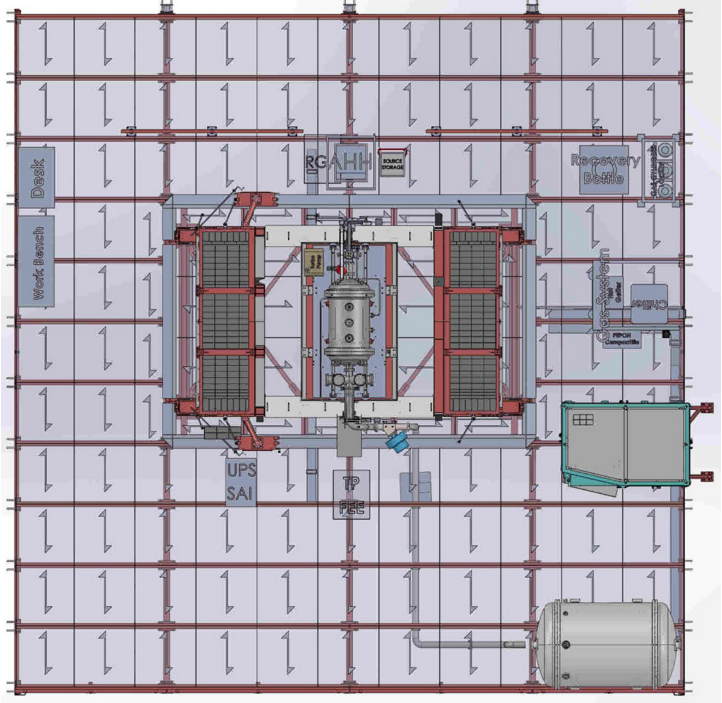
\includegraphics[width=0.7\textwidth, ]{img2/WorkingPlatform.png}}
        \caption{\textit{Layout of the NEXT working platform.}}
        \label{fig.WP}
    \end{center}
\end{figure}

\begin{figure}[hpt!]
    \bigskip
    \begin{center}\leavevmode
        \rotatebox{0}{
        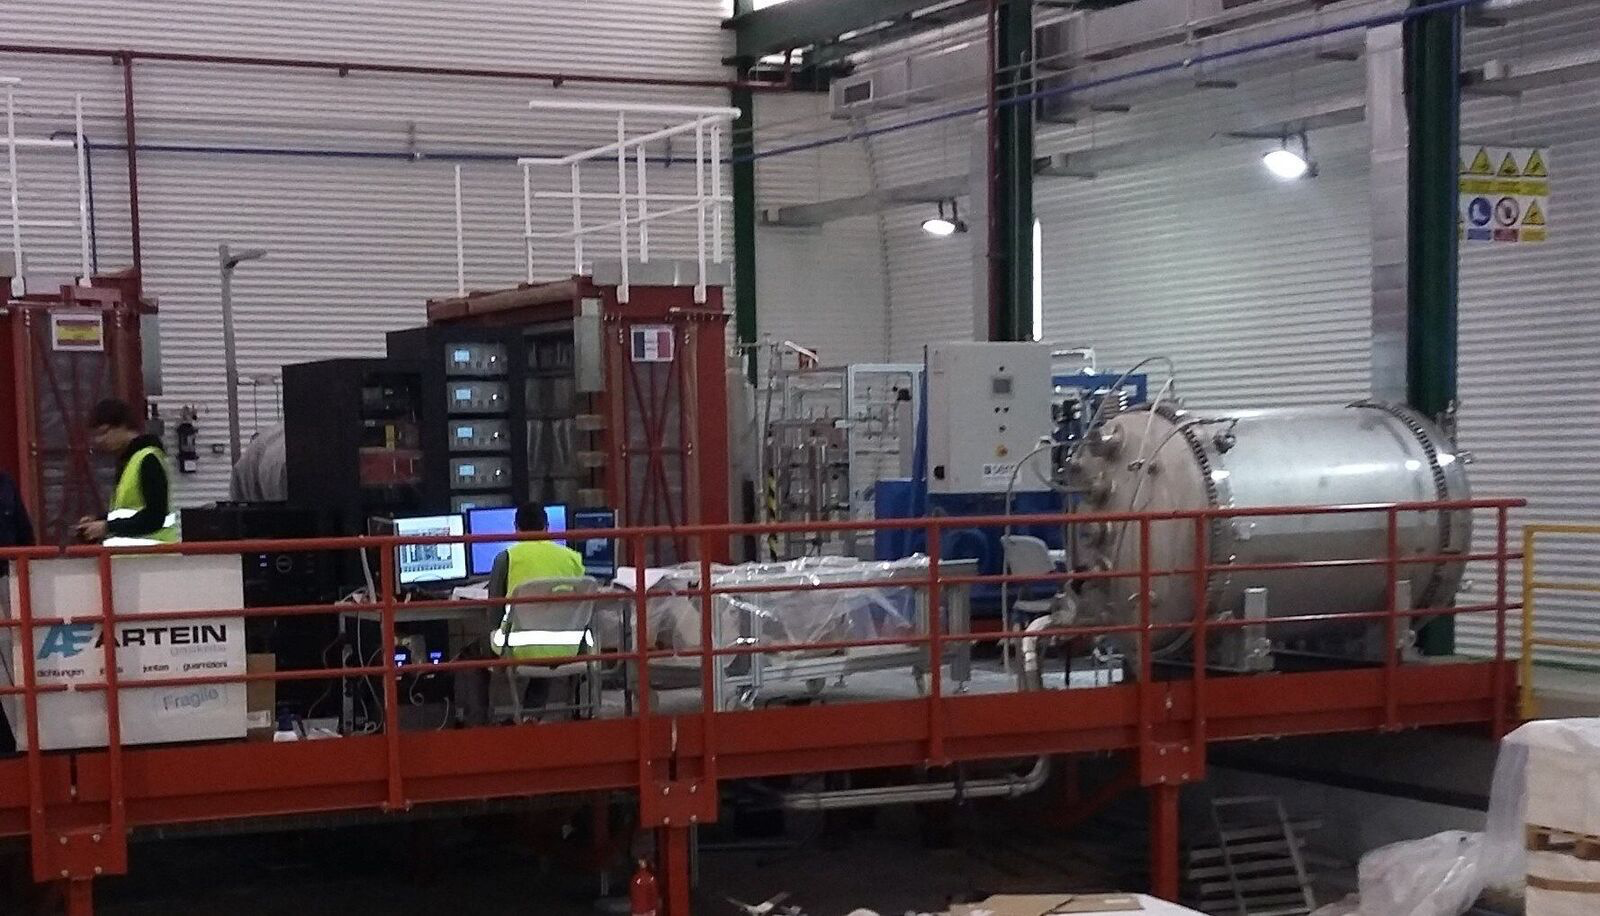
\includegraphics[width=0.7\textwidth, ]{img2/PictureWP.png}}
        \caption{\textit{A picture of the NEXT working platform (April, 2016).}}
        \label{fig.WPP}
    \end{center}
\end{figure}

%
%
%\begin{figure}[hpt!]
%    \bigskip
%    \begin{center}\leavevmode
%        \rotatebox{0}{
%        \includegraphics[width=\textwidth, ]{GasSystemAndInfrastructures/IMG/F2.png}}
%        \caption{\textit{The NEXT working platform, empty}}
%        \label{fig:F2:F2}
%    \end{center}
%\end{figure}
%


\begin{figure}[hpt!]
    \bigskip
    \begin{center}\leavevmode
        \rotatebox{0}{
        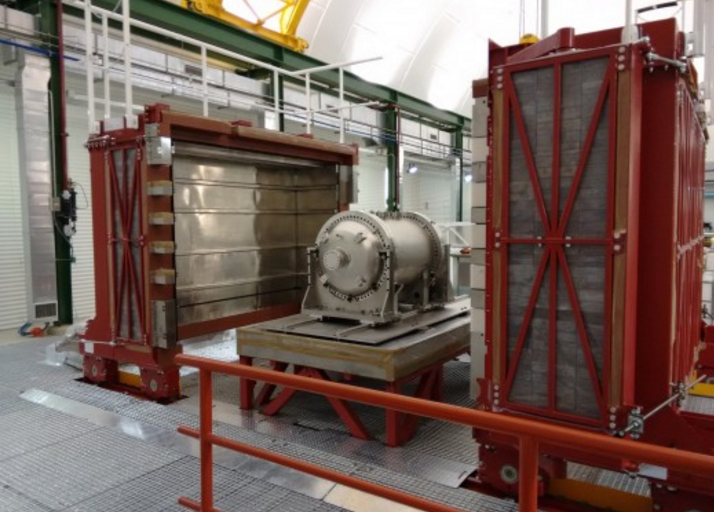
\includegraphics[width=0.7\textwidth, ]{img2/LeadCastleWithNew.png}}
        \caption{\textit{The lead castle in the open position. The NEW apparatus sits on top of the seismic pedestal, which is anchored to the floor via isolating seismic blocks.}}
        \label{fig.LCWN}
    \end{center}
\end{figure}

%\begin{figure}[hpt!]
%\centering
%\includegraphics[height=8cm]{img/SeismicPedestal.pdf}
%\caption{A 3D view of the Seismic Pedestal (SP).} \label{fig:seismicPedestal3D}
%\end{figure}
%


%\begin{figure}
%\centering
%\includegraphics[height=12cm]{img/InfraStruc.pdf}
%\caption{The NEXT infrastructures: (a) The pressure vessel, hosting the detector; (b) the lead castle shield in its open configuration; (c) seismic platform; (d) working platform; (e) gas purification system; (f) emergency gas vent tank; (g) data acquisition system; (h) other systems.} \label{fig:Infrastructure}
%\end{figure}
%
%\begin{figure}
%\centering
%\includegraphics[height=12cm]{img/InfraStruc_2.pdf}
%\caption{The NEXT-100 infrastructures (top view) showing the overall dimensions of the installation.} \label{fig:Infra2}
%\end{figure}


\subsection{Gas system}

\begin{figure}[hpt!]
    \bigskip
    \begin{center}\leavevmode
        \rotatebox{0}{
        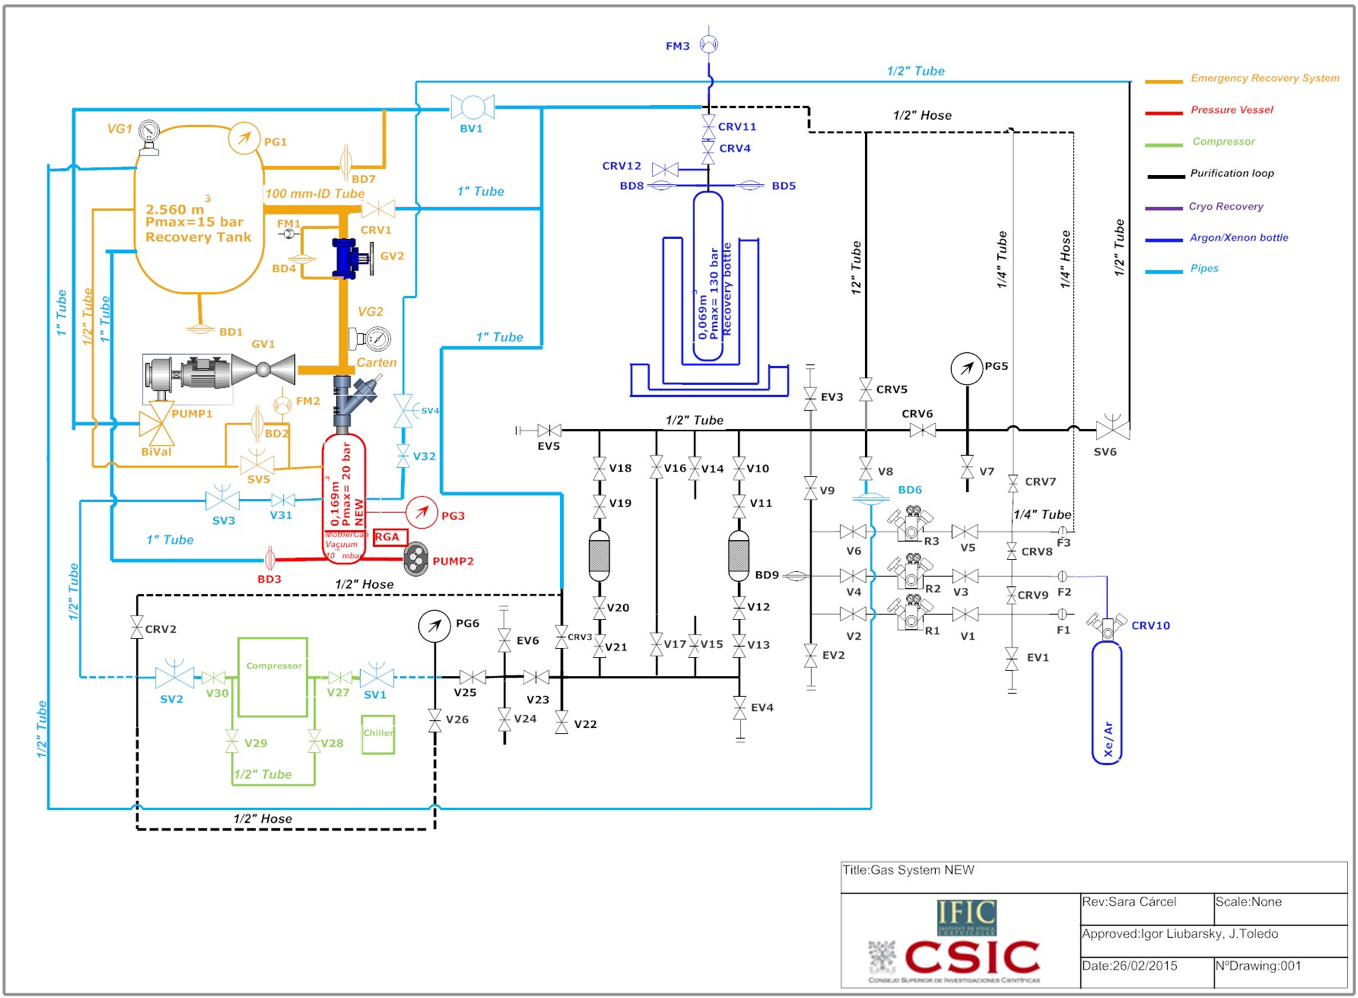
\includegraphics[width=\textwidth, ]{img2/GasSystem.png}}
        \caption{\textit{Schematic of the NEW/NEXT Gas System.}}
        \label{fig.GasSystem}
    \end{center}
\end{figure}

The goal of the gas system, common to the NEW and NEXT-100 detectors, is to purify the xenon, reducing the traces of gases such as ${\rm O_2, CO_2,CO, H_2, N_2, CH_4}$ and water vapour to less than one part per billion (ppb). Both NEW and NEXT-100 will operate with natural xenon and enriched xenon. The gas will be maintained at room temperature and 10--15 bar pressure inside the detector(s). The gas system has been designed to avoid significant losses of xenon under all foreseeable circumstances.

%\begin{figure}[hpt!]
%    \bigskip
%    \begin{center}\leavevmode
%        \rotatebox{0}{
%        \includegraphics[width=\textwidth, ]{img/Gas2.png}}
%        \caption{\textit{Drawing showing the main components of the NEXT gas sytem.}}
%        \label{fig.gas2}
%    \end{center}
%\end{figure}

Figure \ref{fig.GasSystem} shows a schematic of the gas system. Its main components are:  

\begin{itemize}
\item Emergency recovery system.
\item Pressure vessel (NEW or NEXT-100). 
\item Compressor (recirculation pump).
\item Purification loop (hot and cold getters).
\item Cryo-recovery system.
\item Argon/xenon bottles.
\item Pipes.
\item Control System.
\end{itemize}

The pipes are all plumbed together using 1/2'' and 1'' stainless tube and flexible hoses where mechanical insulation is required. The initial operation of NEW is foreseen to 10 bar, with the possibility to operate at 15--20 bar in 2017. The nominal operation pressure of NEXT-100 is 15 bar. 

\subsubsection*{Emergency recovery tank and ancillary systems}

\begin{figure}[hpt!]
    \bigskip
    \begin{center}\leavevmode
        \rotatebox{0}{
        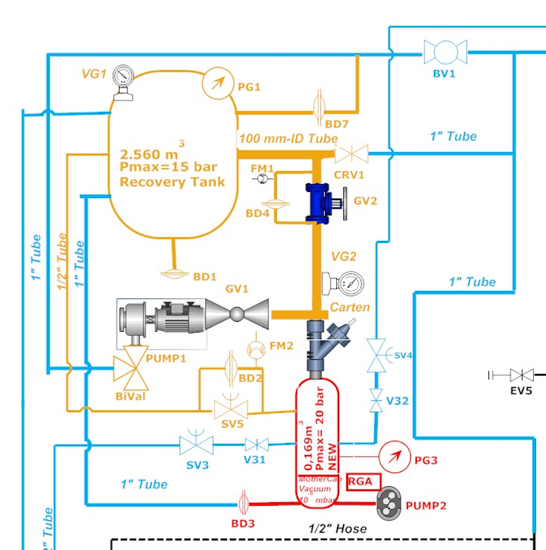
\includegraphics[width=0.55\textwidth, ]{img2/GasER.png}}
        \caption{\textit{Emergency Recovery section of the Gas System}}
        \label{fig.GER}
    \end{center}
\end{figure}


\begin{figure}[hpt!]
    \bigskip
    \begin{center}\leavevmode
        \rotatebox{0}{
        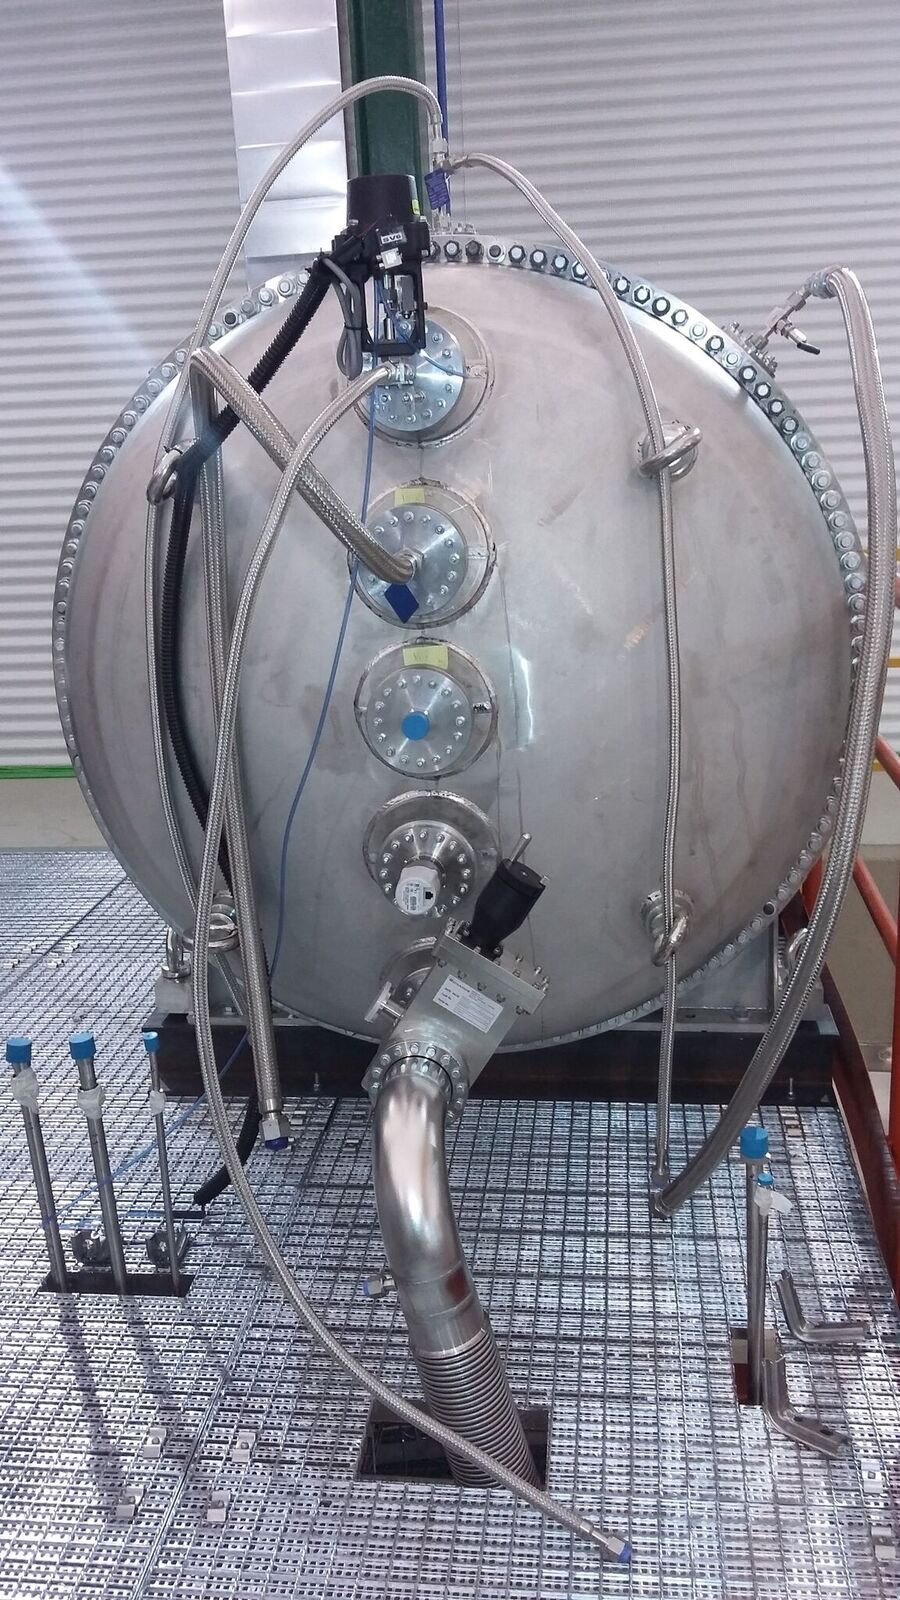
\includegraphics[width=10cm ]{img2/NEXT100AsRecoveryVessel.png}}
        \caption{\textit{The NEXT-100 pressure vessel operating as Emergency Recovery Tank.}}
        \label{fig.N100}
    \end{center}
\end{figure}

\begin{figure}[hpt!]
    \bigskip
    \begin{center}\leavevmode
        \rotatebox{0}{
        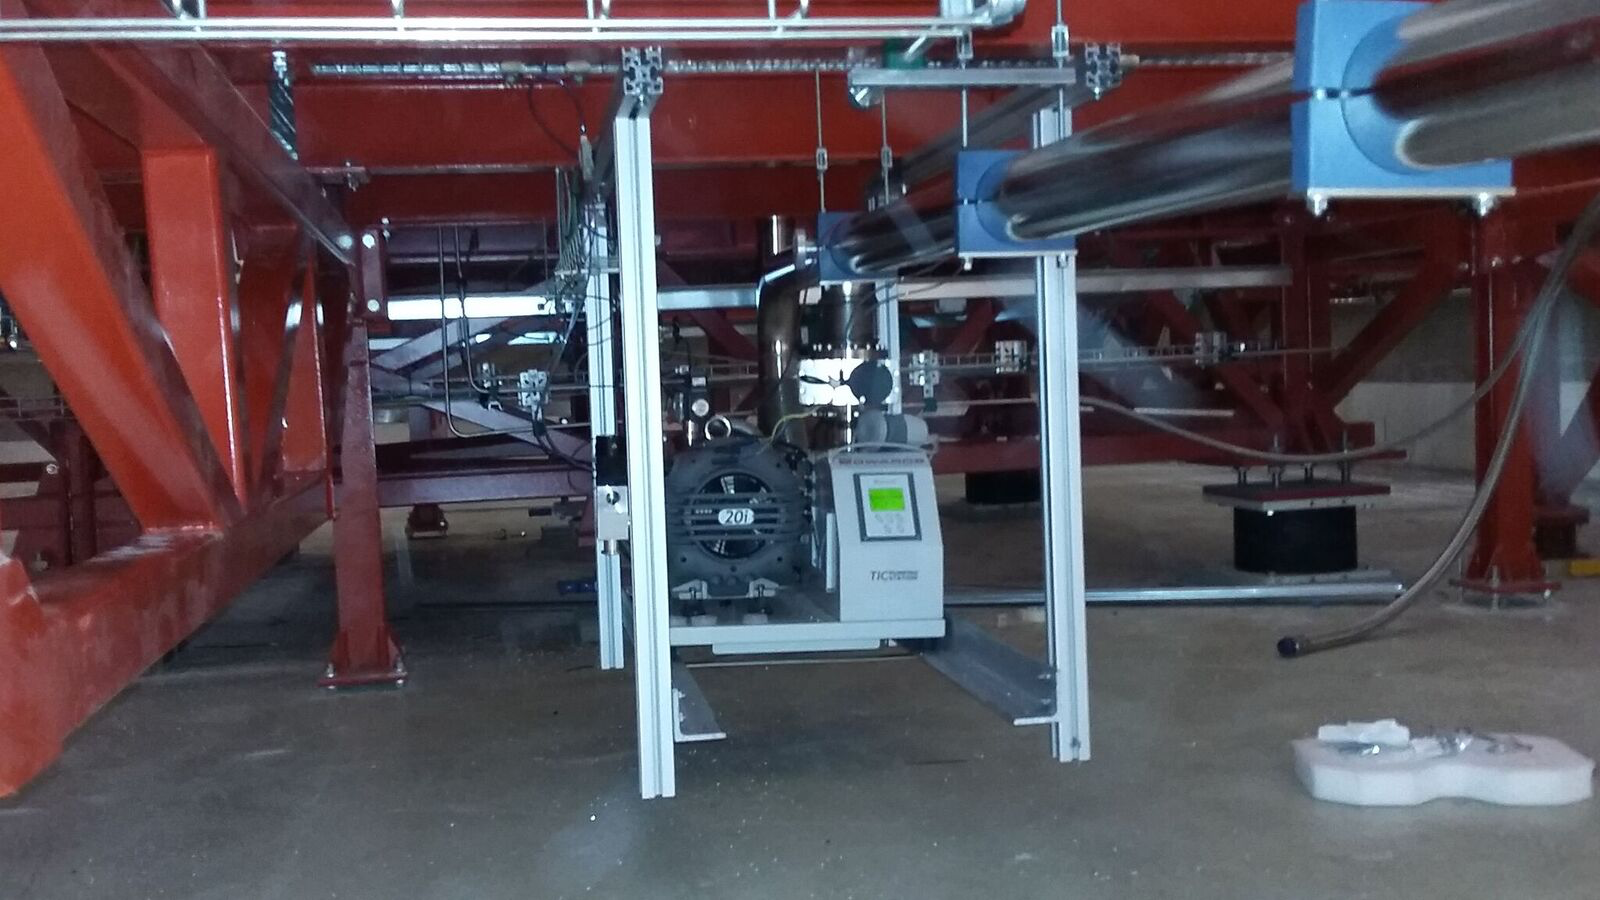
\includegraphics[width=0.45\textwidth, ]{img2/PUMP1.png}
        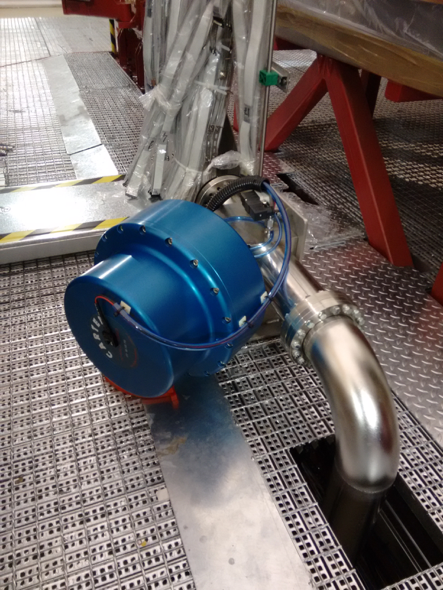
\includegraphics[width=0.45\textwidth, ]{img2/CartenValve.png}
        }
        \caption{\textit{Left:a picture of the vacuum pump (PUMP1) used to keep the recovery tank at a 
        nominal pressure of $10^{-5}$~mbar. The pump is sitting under the working platform. Right: a picture of
        the Carten valve used to separate the pressure side from the vacuum side in the gas system.}}
        \label{fig.P1}
    \end{center}
\end{figure}


The emergency recovery section of the gas system (figure \ref{fig.GER}) is designed to recover gas into a recovery tank in the event of over-pressure in the gas system. During the operation of NEW, the existing pressure vessel of the NEXT-100 experiment (a tank with a volume of 2.560 m$^3$~ made of 316Ti alloy and with CE certification for operation at 15 bar) is reused as a recovery tank (figure \ref{fig.N100}). In order to guarantee that gas is dumped into the recovery tank in the event of over-pressure, the tank is kept during normal operations at $10^{-5}$~mbar. This is done by pumping the tank with the vacuum pump PUMP1 (figure \ref{fig.P1}--left panel)
through a pneumatic-activated guillotine valve (GV1), certified to separate pressure from 
vacuum zones (figure \ref{fig.P1}, right panel). A second manual valve GV2 acts as a backup. A pressure gauge (PG1) and a vacuum gauge (VG1) measure the pressure and vacuum in the recovery tank. A bursting disk installed in the recovery tank (BD1) will break at 5 bar, avoiding any over-pressure in the system. Notice that a pressure of 10 bar in the NEW vessel translates into a pressure of $\sim$1 bar in the recovery tank, and therefore 5 bar provides a wide tolerance margin.   
%A second disk, BD7, will break at 3 bar. The disk function is to avoid an over pressure over 30 bar in the gas system. In practice, BD7 is relevant only in case that BV1 is opened by mistake when there is pressure in the purification loop. 

%In normal operations, the vacuum pump (PUMP1) is pumping the recovery tank and GV1 is opened. The valve is automatically controlled by the Slow Control System and to be open needs a pneumatic pressure of 4.5-5 bar and a voltage of 24 VDC. This implies that the valve closes in failure (electrical of pneumatic shutdown at the experiment or the LSC). Also, if an emergency condition (need to recover the gas) arises, PUMP1 is turned off and GV1 closes. Emergency conditions are normally triggered by excess pressure in the NEW pressure vessel. In this case, the Carten Valve opens up and as GV2 is always open, the gas will evacuate to the tank through the safety evacuation line.A second pneumatic valve, SV6 is controlled by the Slow Control System and will open up in the event of excess pressure. If both the Carten valve and SV6 fail, disk BD2 will burst at 13 bar. 

\subsubsection*{Pressure vessel}

\begin{figure}[hpt!]
\centering
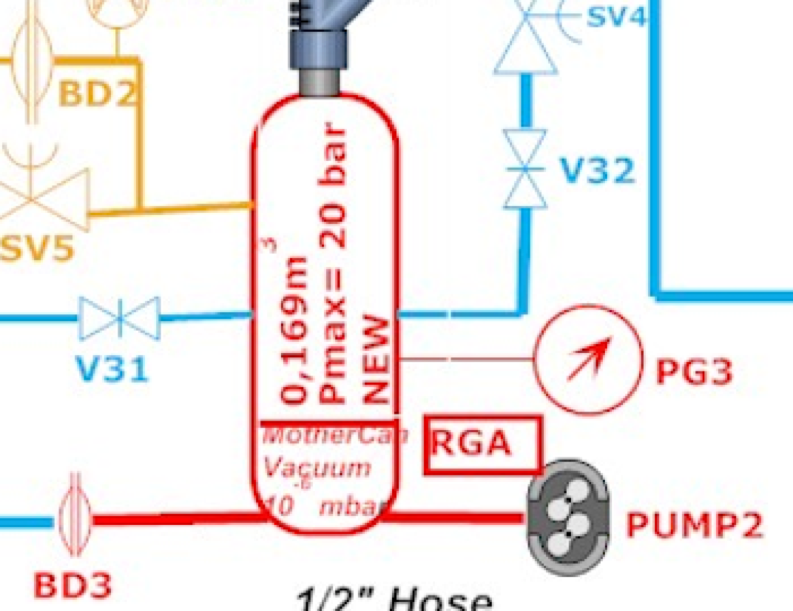
\includegraphics[height=6cm]{img2/PVGS.png}
\caption{A diagram of the pressure vessel section of the gas system.} \label{fig.pvgs}
\end{figure}

Figure \ref{fig.pvgs} shows the pressure vessel section of the gas system. Currently, the pressure vessel is that of NEW, 
a tank with a volume of 0.169 m$^3$~ fabricated with a radiopure steel-titanium alloy (316Ti) and certified to operate up to 20 bar. Inside the pressure vessel there is region (called the pressure side) held at high pressure (10--15 bar) and a region held at modest vacuum $10^{-5}--10^{-6}$~mbar (called the vacuum side). The two regions are separated by a sealing copper plate (called the mother-can), which is described in more detail in section \ref{sec.new}. 

To reach the desired vacuum level in the vacuum side, PUMP2 is switched on. In the event of a breach between the
pressure and the vacuum side PUMP2 is switched off by the Slow Control System. A bursting disk (BD3) will break at 3 bar, preventing the PMTs from being damaged, and the gas will be evacuated to the emergency recovery tank. A mass spectrometer (also called the RGA, short for Residual Gas Analyser)
detects the partial pressure of gas in the vacuum side.


\subsubsection*{Recirculation compressor}

%\begin{figure}[hpt!]
%\centering
%\includegraphics[height=12cm]{img/Pump.pdf}
%\caption{Schematics of the SERA recirculation compressor, chosen by NEXT.} \label{fig:pump}
%\end{figure}

\begin{figure}[hpt!]
\centering
\includegraphics[height=8cm]{img2/Compressor.png}
\caption{A picture of the compressor.} \label{fig.sera}
\end{figure}

The most vulnerable component of the gas system is the compressor, which acts as a re-circulation pump. The enriched xenon is very expensive and therefore the pump to move the gas through the re-circulation loop must have sufficient redundancy to minimise the probability of failure and leakage. Furthermore, to preserve the purity of the gas all metal-to-metal seals must be used. 

Figure \ref{fig.sera} shows a picture of the compressor chosen for NEXT, manufactured by the SERA company, in Germany. The pump is made with metal-to-metal seals on all the wetted surfaces. The gas is moved through the system by a triple stainless steel diaphragm, ensuring a negligible probability of catastrophic failure (gas liberated to the atmosphere). Between each of the diaphragms there is a sniffer port to monitor for gas leakages. In the event of a leakage, automatic emergency shutdown can be initiated. 

\subsubsection*{Getters}

\begin{figure}[hpt!]
\centering
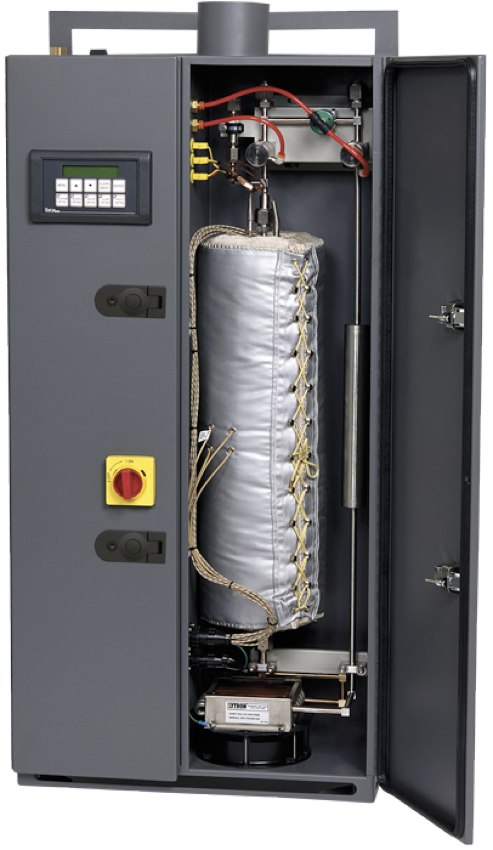
\includegraphics[height=8cm]{img2/HotGetter.png}
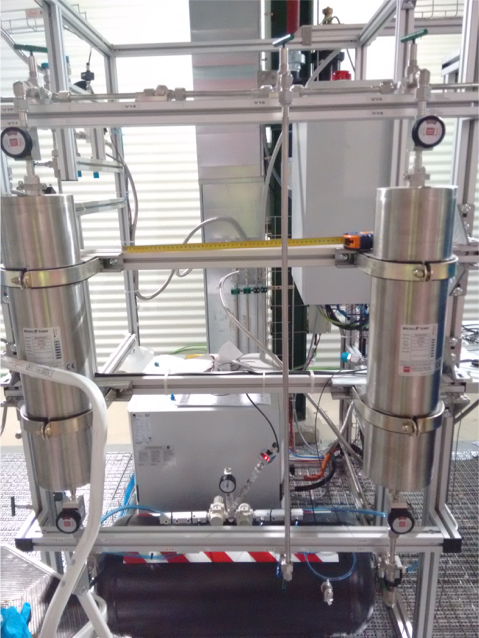
\includegraphics[height=8cm]{img2/ColdGetters.png}
\caption{Top: The PS4-MT50 SAES hot getter. Bottom: detail of the gas system with the cold getters already installed.} \label{fig:getter}
\end{figure}


Hot and cold getters (figure \ref{fig:getter}) are used to purify the gas. The gas is circulated first through cold getters in order to eliminate water vapor, as well as other electronegative (oxygen and carbon dioxide) impurities. Once the gas is sufficiently clean the hot getter is switched on to remove nitrogen and methane and further purify the gas to less than 1 ppb. 

\subsubsection*{Recirculation loop and cryo-recovery }

\begin{figure}[hpt!]
\centering
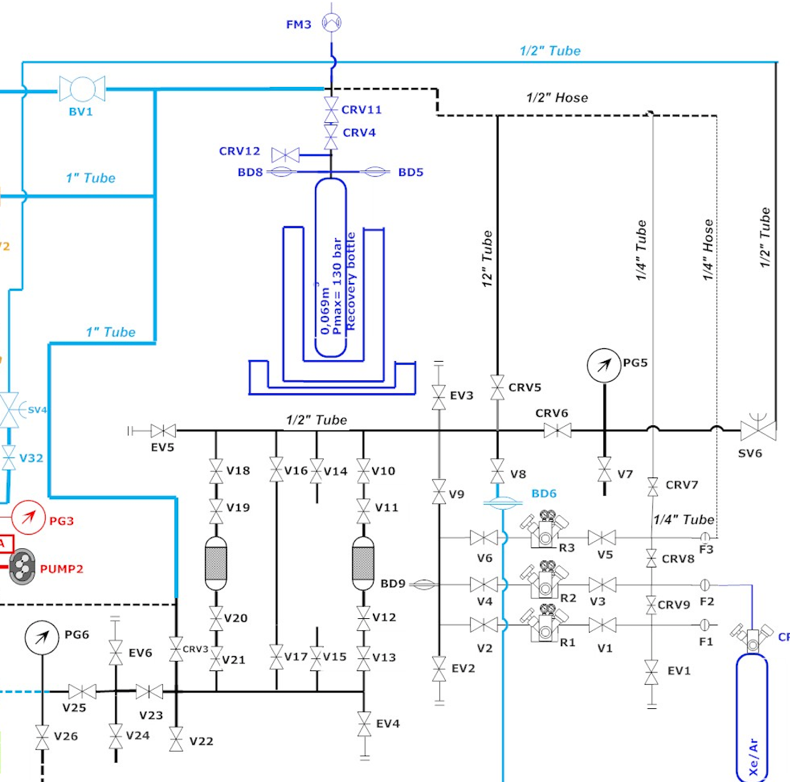
\includegraphics[height=8cm]{img2/Recirculation.png}
\caption{A schematic of the recirculation loop and cryo-recovery part of the gas system.} \label{fig.ct}
\end{figure}

\begin{figure}[hpt!]
    \bigskip
    \begin{center}\leavevmode
        \rotatebox{0}{
        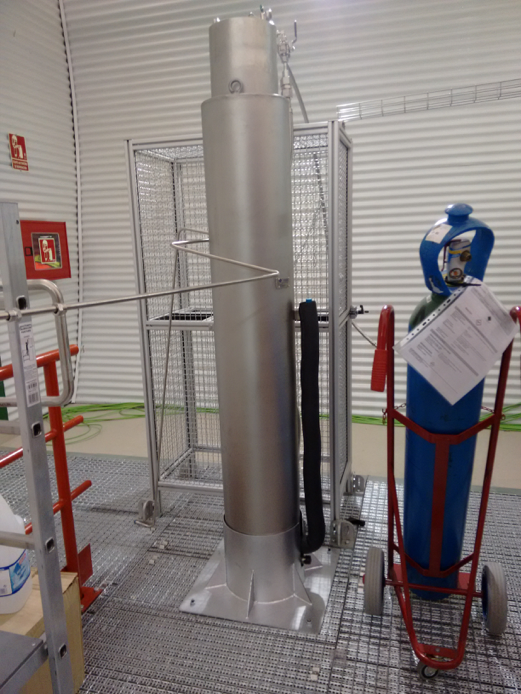
\includegraphics[width=8cm]{img2/CryoBottle.png}}
        \caption{\textit{The cryo-recovery system consists of a large bottle sitting inside an open Dewar. Cooling the bottle with liquid nitrogen reclaims the xenon circulating in the system.}}
        \label{fig.CB}
    \end{center}
\end{figure}

Figure \ref{fig.ct} shows the recirculation loop. The gas enters the system from the pressure bottle, through a regulator and circulates through cold and/or hot getters ( \ref{fig:getter}), under the action of the compressor 
(figure \ref{fig.sera}). To recover the gas under normal conditions a bottle sitting inside an open Dewar (figure \ref{fig.CB}) is used. 

\subsubsection*{Summary}
 
The needed infrastructure for the NEXT experiment has been completed during 2015 and the first quarter of 2016. The gas system is now in the final commissioning phase, and ready to pass the tests needed for underground operation certification in the next few weeks. Start-of-operations is foreseen for May, 2016. 

%\newpage
\section{The NEW detector}
\label{sec.new}


\begin{figure}[hpt!]
\centering
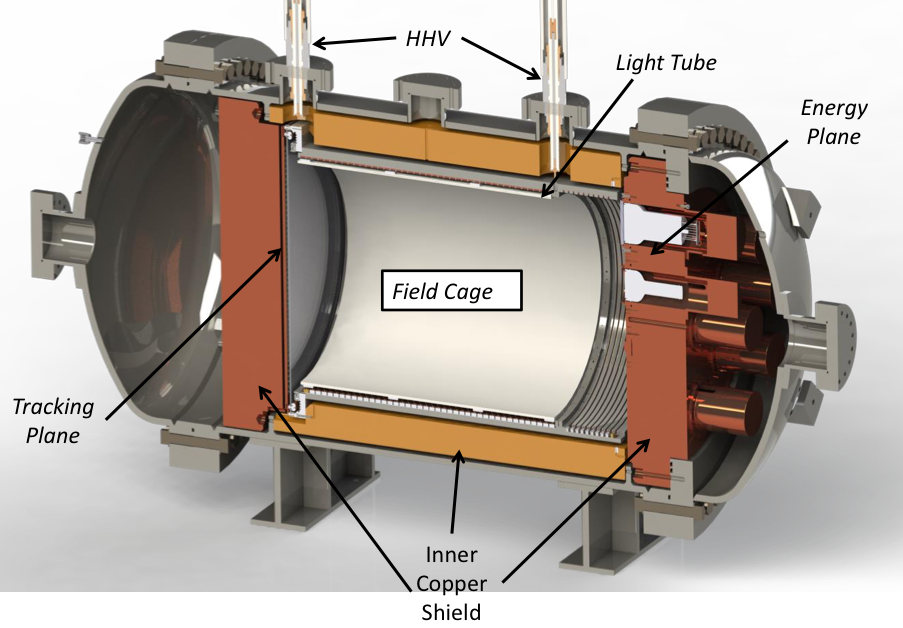
\includegraphics[height=8cm]{img2/NEWMay20163D.png}
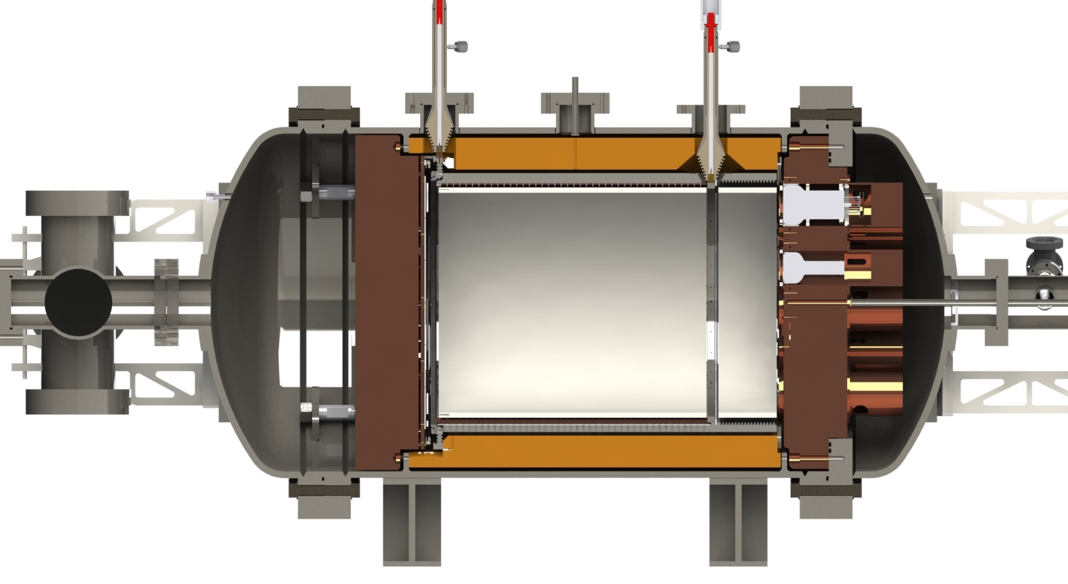
\includegraphics[height=8cm]{img2/NEWMay2016.png}
\caption{Top: a 3D drawing of the NEW detector, showing its main parts. Bottom: a lateral view of NEW, including the ancillary equipment used to extract the signals from the energy plane and the tracking plane.  } \label{fig:NewOverview}
\end{figure}

\begin{figure}[hpt!]
\thisfloatpagestyle{empty}
\centering
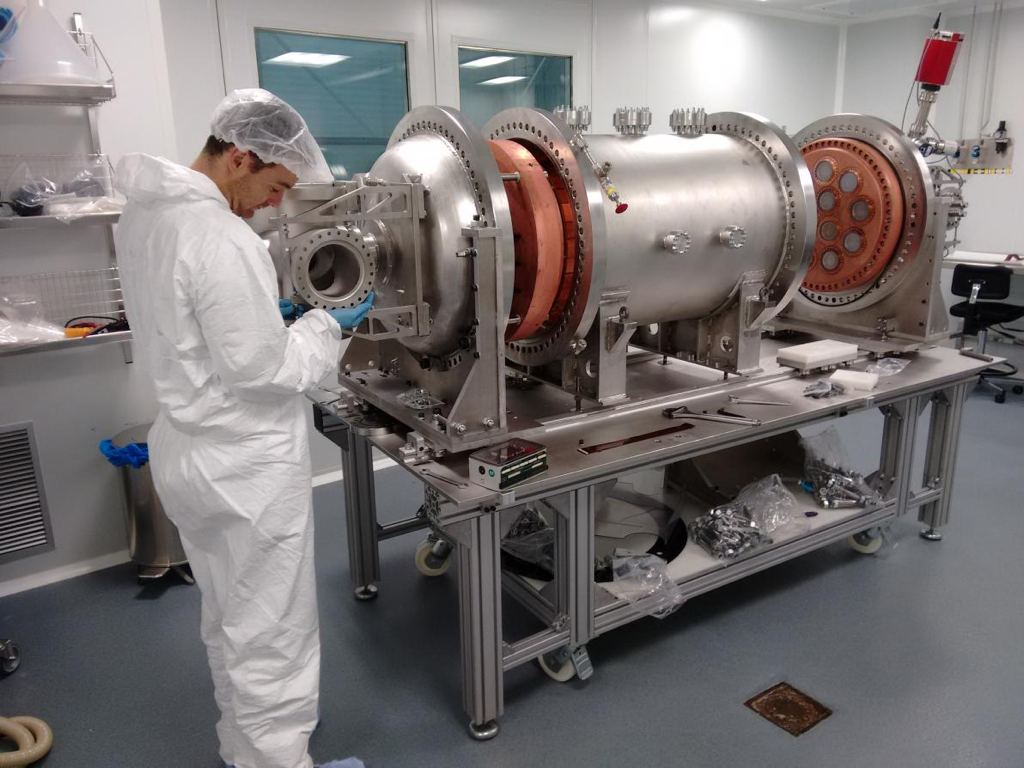
\includegraphics[height=6.5cm]{img2/NewInCRWIthAlberto.png}
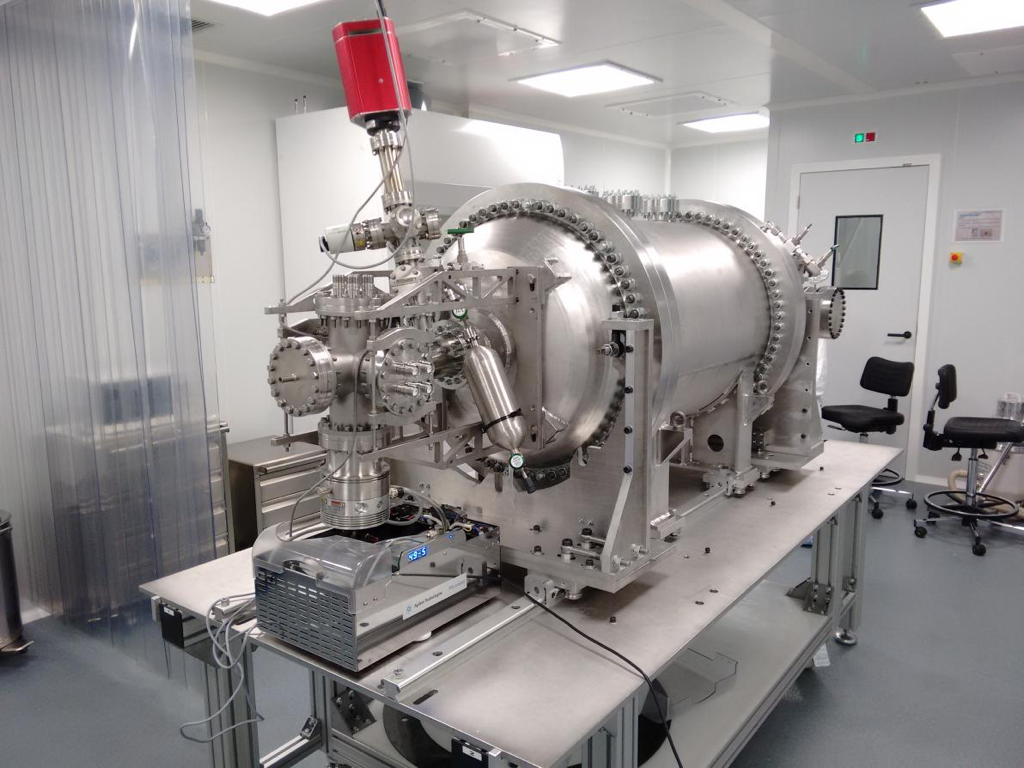
\includegraphics[height=6.5cm]{img2/NewSeenFromEP.png}
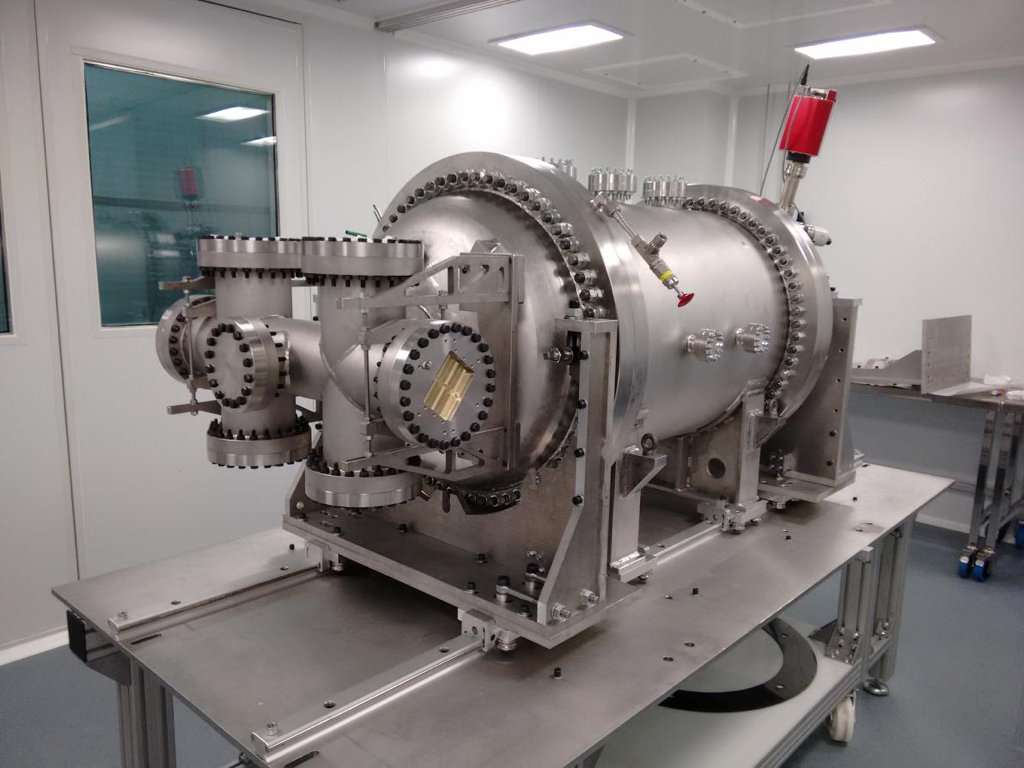
\includegraphics[height=6.5cm]{img2/NewSeenFromTP.png}

\caption{The NEW detector being assembled in the LSC clean room in 2015. Top: A picture from the side, showing the two end-caps open. The thick copper plates supporting the energy plane and the tracking plane are clearly visible. Middle: the detector seen from the Energy Plane side. The EP ``cross'' holds the feedthroughs (each side of the cross allows for the extraction of 4 PMT signals) and also connects to the pump used to make vacuum in the vacuum side of the detector (in the picture the pump displays the level of vacuum achieved, $4.9 \times 10^{-5}$~mbar). The RGA is also clearly visible. Bottom. The detector seen from the tracking plane side. The TP ``spaceship" holds the TP feedthroughs.} \label{fig.New}
\end{figure}

The NEW detector, shown in figure \ref{fig:NewOverview}, is the first stage of the NEXT experiment. The NEW pressure vessel and field cage
 dimensions are roughly 1:2 with respect to those of NEXT-100. It deploys 20 \% of the NEXT-100 sensors and the xenon mass is about 10 kg at 15 bar. 

The primary goal of NEW is to provide an extra step in the construction of the NEXT-100 detector that allows for the validation of the technological solutions proposed in the NEXT-100 technical design report (TDR)\cite{Alvarez:2012haa}. In addition, NEW will permit a measurement of the energy resolution at high energy, and the precise characterisation of the 2-electron topological signature, by measuring the \bbtnu\ mode. Last but not least, NEW will permit a realistic assessment of the NEXT background model before the construction of the NEXT-100 detector. 

Figure \ref{fig.New} shows the assembly of NEW at the LSC clean room during 2015. The detector has three main parts called the {\em Energy Plane} (EP), {\em Tracking Plane} (TP) and {\em Field Cage} (FC). The EP and TP are already installed in the NEW pressure vessel. The FC will be installed during the first week of May 2016.

%\subsection{Pressure Vessel}
%The NPV has been manufactured by the company TRINOS vacuum system, with the same steel alloy selected for the NEXT-100 detector. The fabrication of the NPV was made possible, at zero cost for the NEXT collaboration, thanks to a CEDETI grant. Figure \ref{fig.npv} shows the pressure vessel and one of the torispherical heads. 
%
%\begin{figure}
%\begin{center}
%\includegraphics[width=0.80\textwidth]{img/NewPV.pdf}
%\includegraphics[width=0.80\textwidth]{img/NewPVHead.pdf}
%\end{center}
%\caption{\label{fig.npv} The NEW Pressure Vessel (NPV).}
%\end{figure}
%
%With an internal diameter of 64 cm and a length of 950 cm, the dimensions of the NPV are intermediate between NEXT-DEMO and NEXT-100. The NPV can hold pressures of up to 50 bar.
%
%\begin{figure}
%\centering
%\includegraphics[height=8cm]{img/PVInTable.pdf}
%\caption{The NEW detector: still a tabletop experiment.} \label{fig:PVInTable}
%\end{figure}
%
%Figure \ref{fig:PVInTable} shows the NPV sitting in a support platform. The platform will be first tested at IFIC, then moved to the LSC. The drawing illustrates the access to the detector. Each head has attached one of the photosensor detection systems (energy plane and tracking plane). 
%

\subsection{Energy Plane}
\begin{figure}[hpt!]
\centering
%\includegraphics[height=8cm]{img/NEPLateralView.pdf}
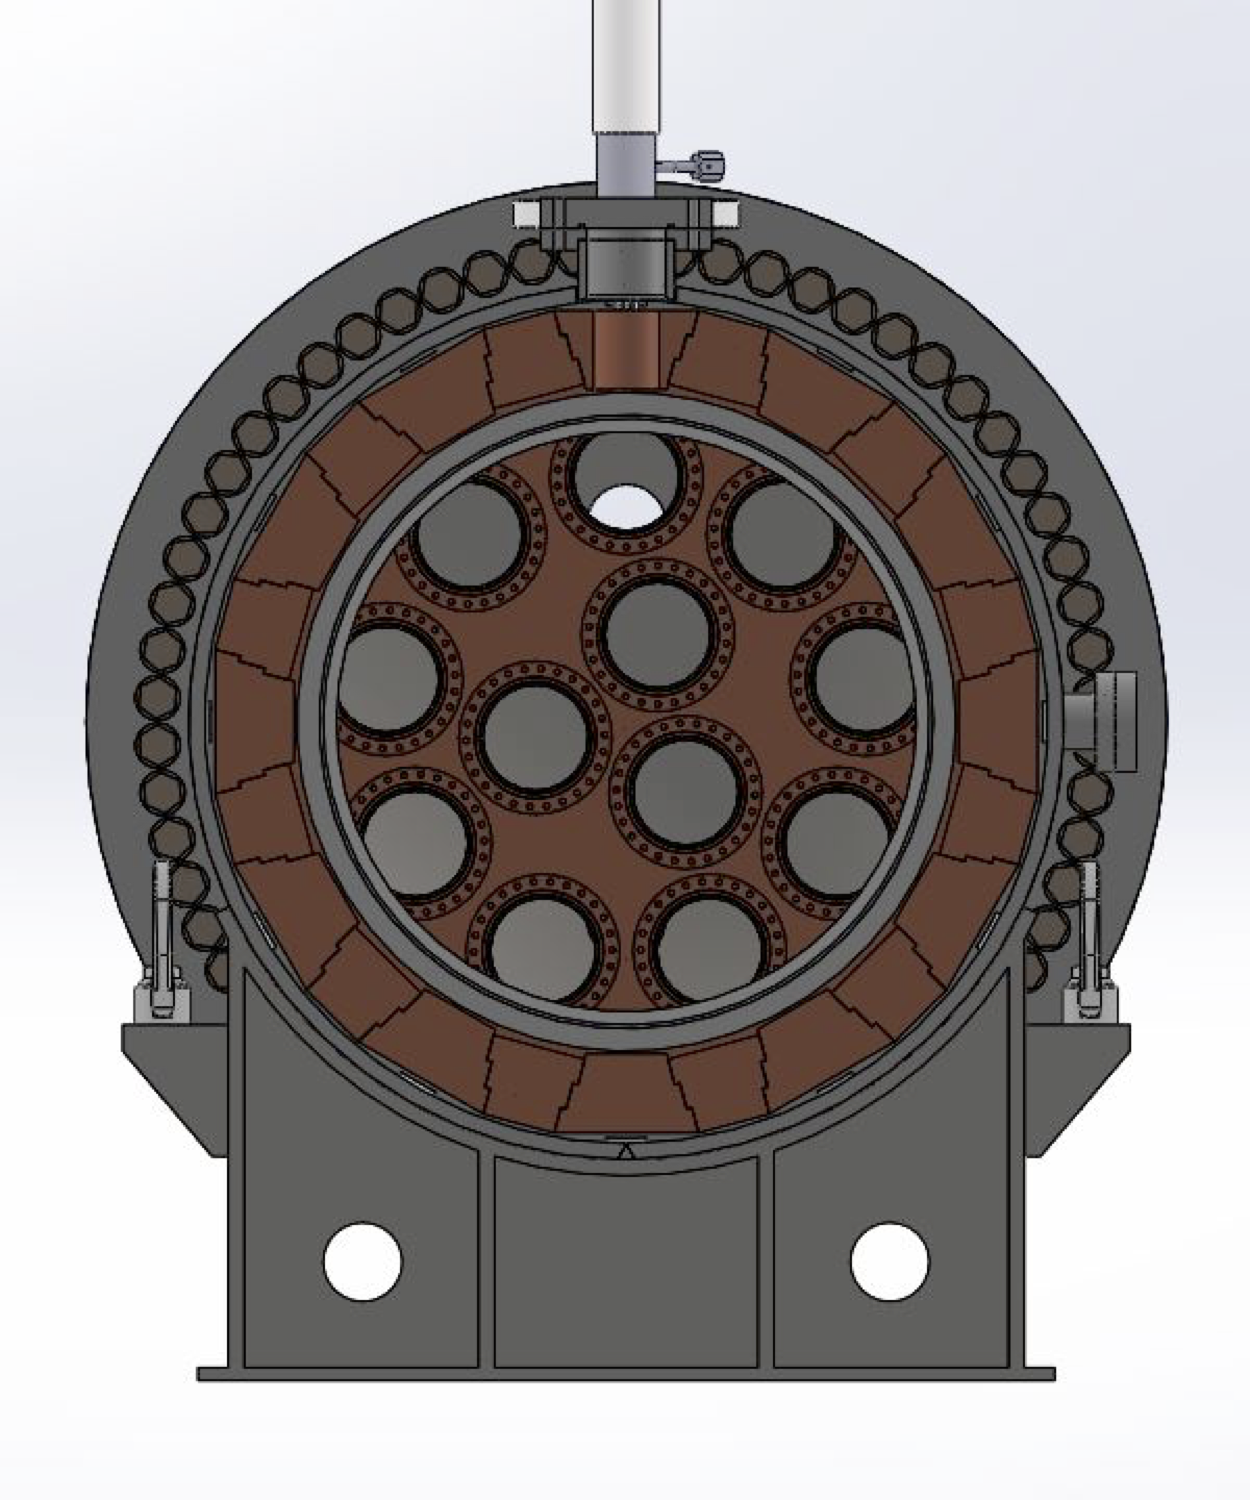
\includegraphics[height=8cm]{img2/NEPFrontView.png}
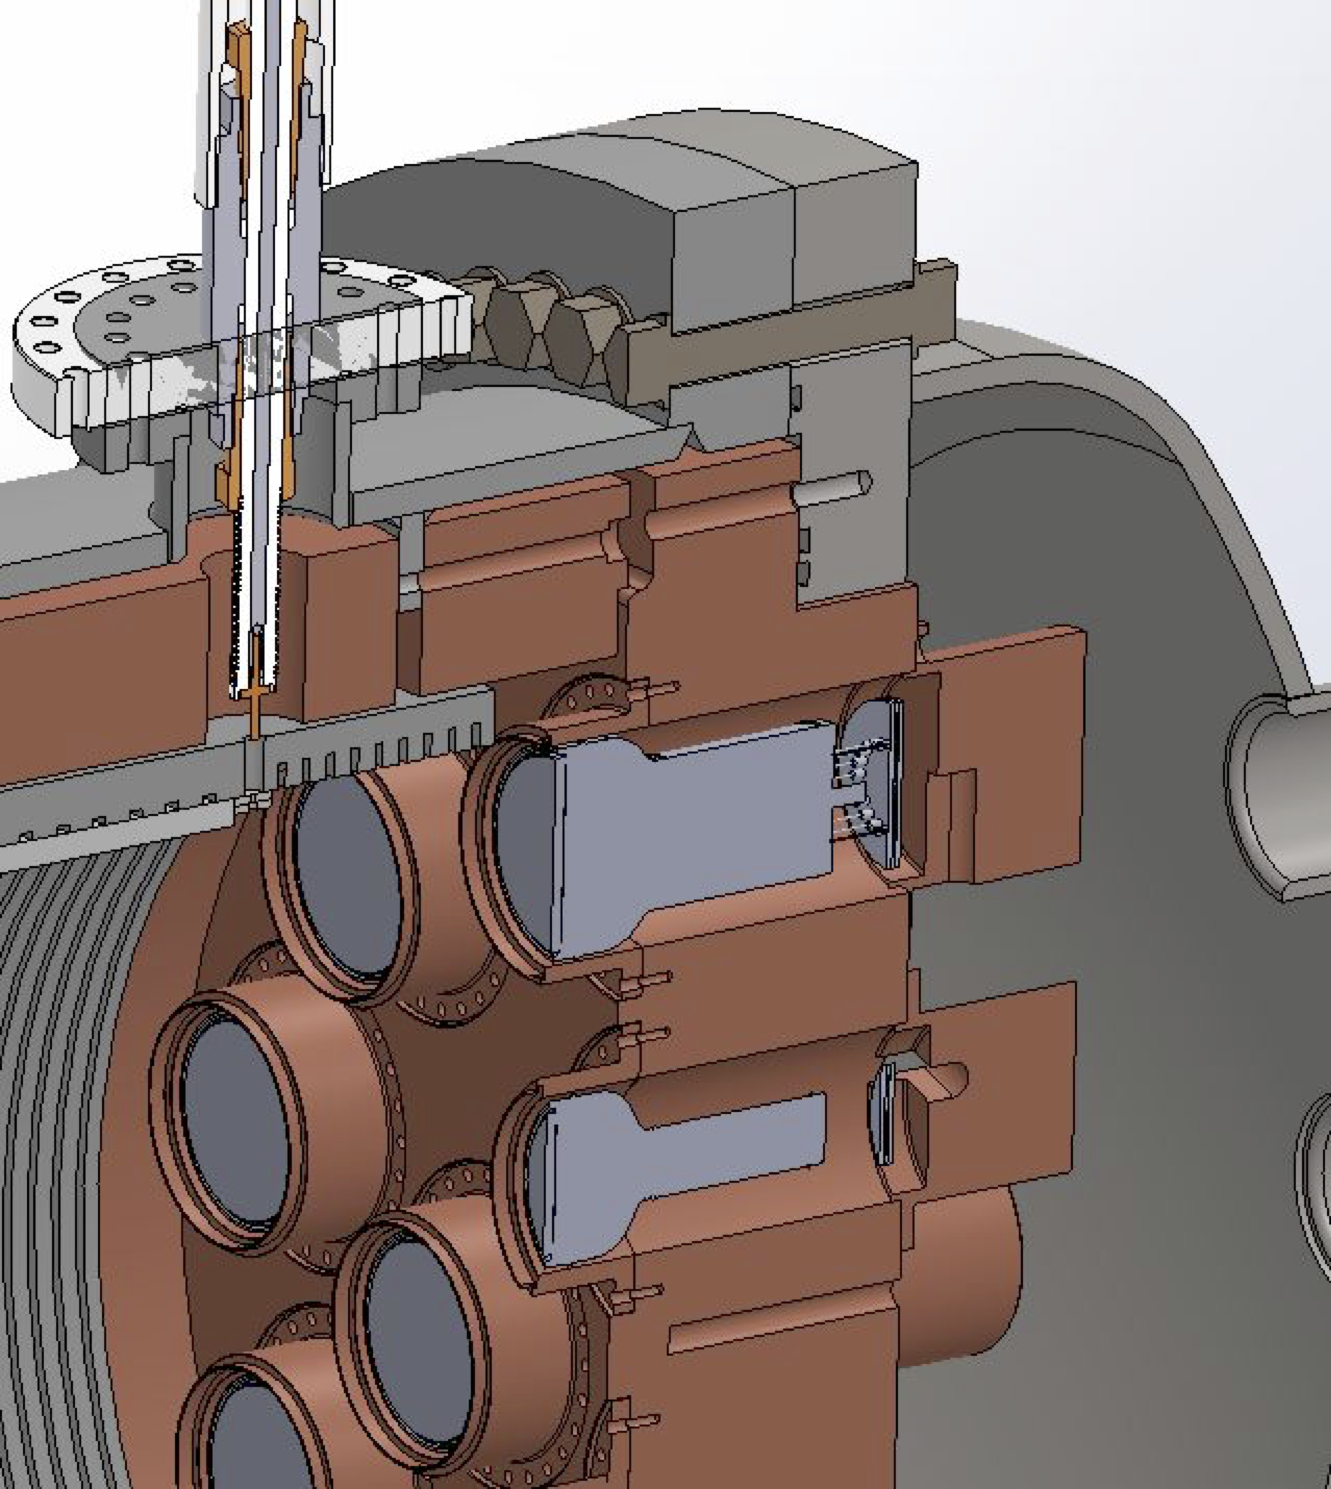
\includegraphics[height=8cm]{img2/NEPDetail.png}
\caption{The NEW energy plane (EP) deploying 12 PMTs operating in vacuum
and coupled to the field cage volume by sapphire windows coated with TPB. Top: front view. Bottom: Detail showing the sapphire windows and the PMT enclosures (aka cans) terminated in thick copper caps for radiation shielding.} \label{fig:NEP}
\end{figure}


\begin{figure}[hpt!]
\centering
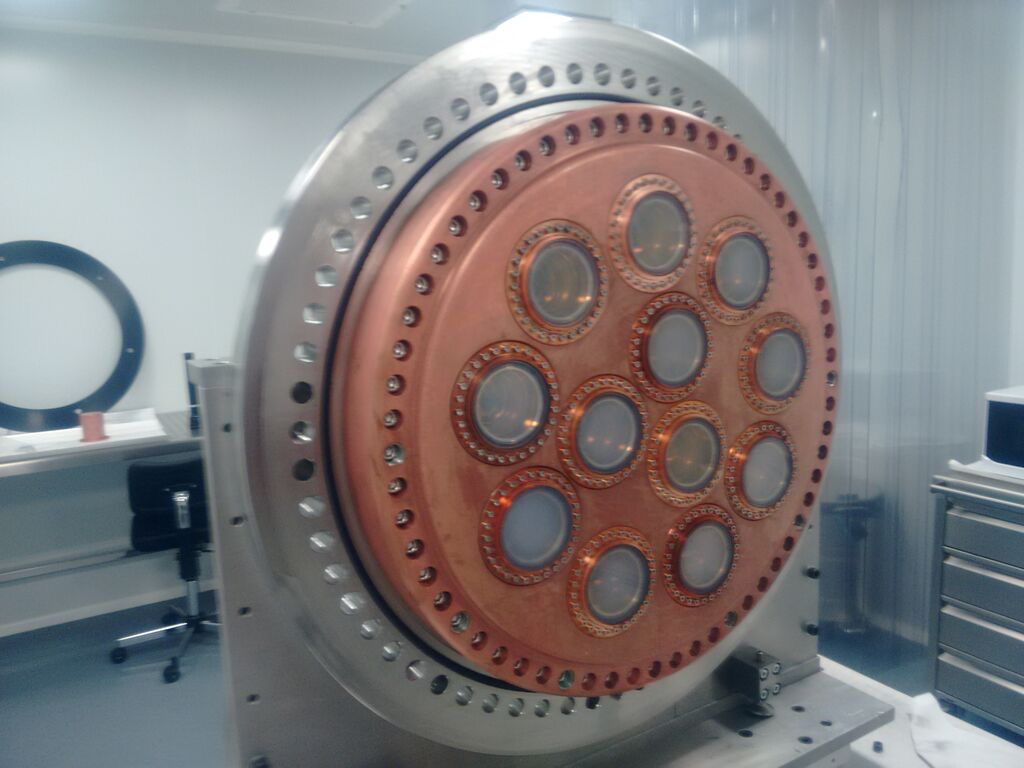
\includegraphics[height=8cm]{img2/EP_ENDCUP.png}
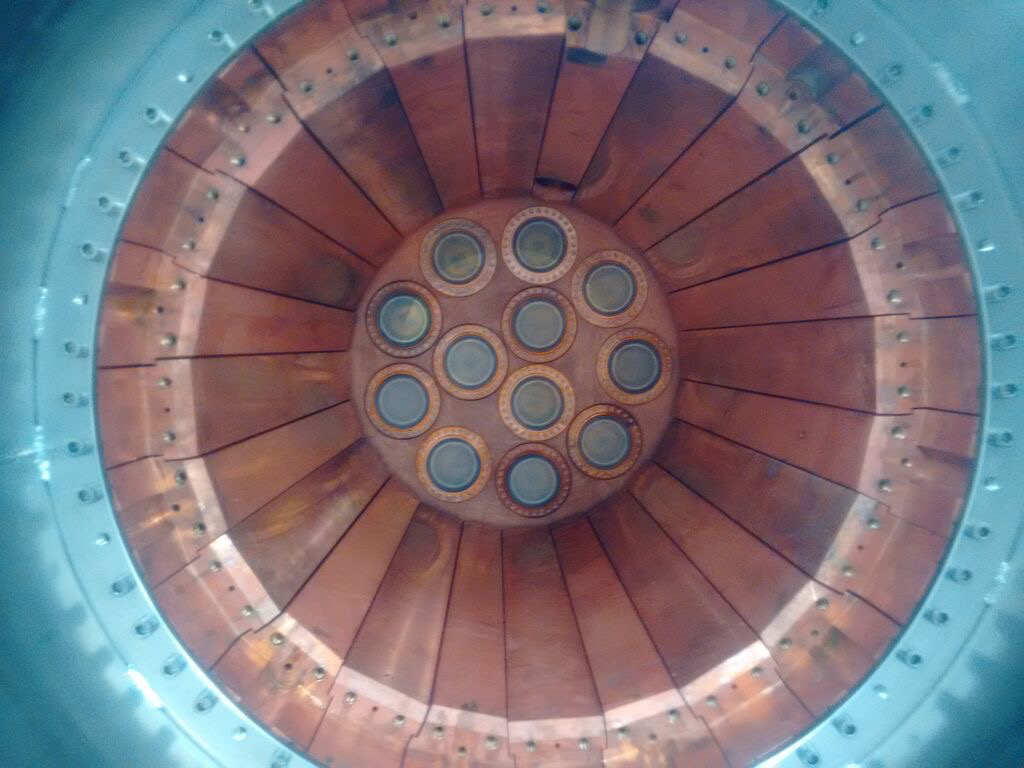
\includegraphics[height=8cm]{img2/EPI.png}
\caption{Assembly of the EP in 2015. Top: The end-cap plate (mother-can) with the sapphire windows already installed. Bottom: the energy plane seen from the tracking plane side. The picture also shows the cooper bars from the inner copper shielding, intended to attenuate the external radiation. } \label{fig.EPA}
\end{figure}

The energy plane is shown in figure \ref{fig:NEP} and pictures of the installation in 2015 are shown in
figure \ref{fig.EPA}. The EP 
consists of a 11 cm thick copper support plate (called the mother-can) with 12 copper cans
covered with brazed sapphire windows fixed to the front of the plate. The
set-up as a whole seals the pressure vessel from the PMT-region,
which is held at vacuum levels of
$<10^{-5}$~mbar. Additional copper shielding fixed to the
vacuum side of the apertures offers further shielding against gammas traversing the PMTs and
entering the detector volume. The 12 Hamamatsu R11410 PMTs are optically coupled to 
the sapphire window using NyoGel OCK-451. The sensors are held in place by a plastic brace and spring.

The PMTs receive high voltage and have their signal extracted via a
shielded, twisted pair cable connected to a feedthrough in the energy-plane head. The distribution of
signal and supply at each individual PMT is controlled via a
Kapton circuit board (base), covered with a
copper cap filled with epoxy and connected to the support plate. The cap acts as a heat sink.


\subsection{Tracking Plane}

\begin{figure}[hpt!]
\thisfloatpagestyle{empty}
\centering
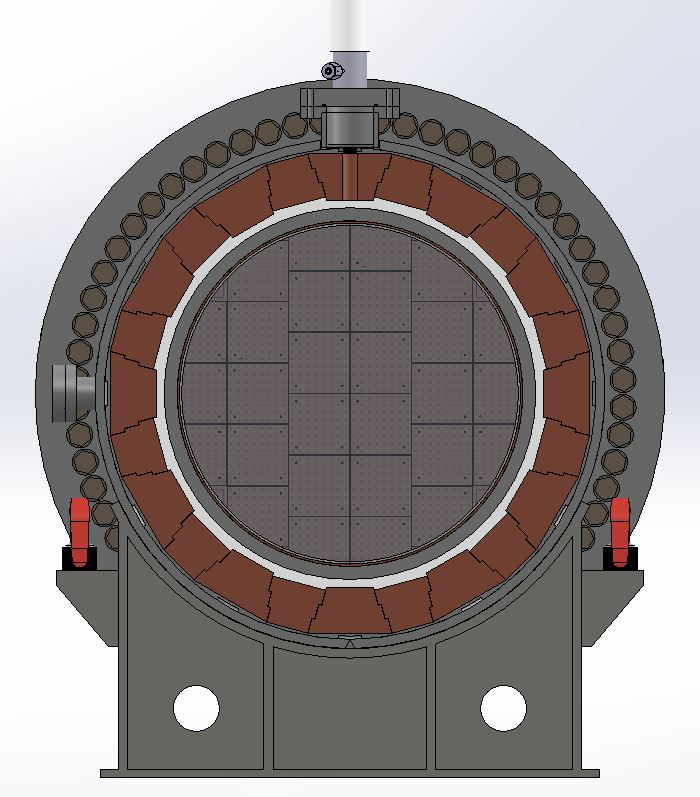
\includegraphics[height=8cm]{img2/TrackingPlane.png}
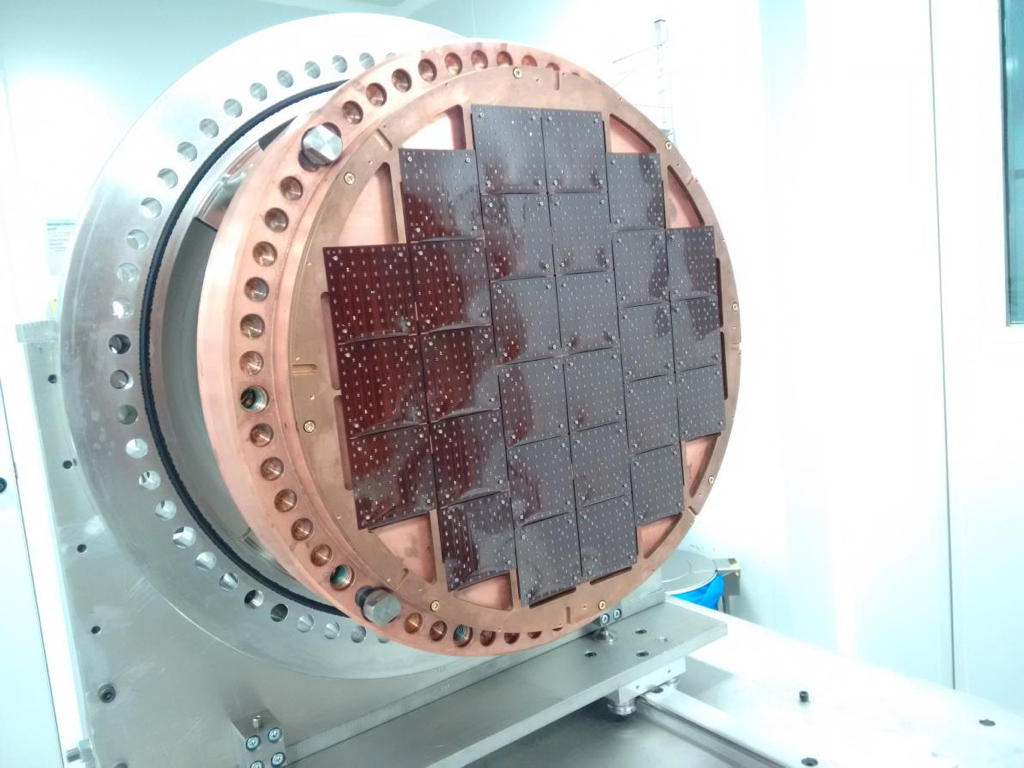
\includegraphics[height=8cm]{img2/TPI1.png}
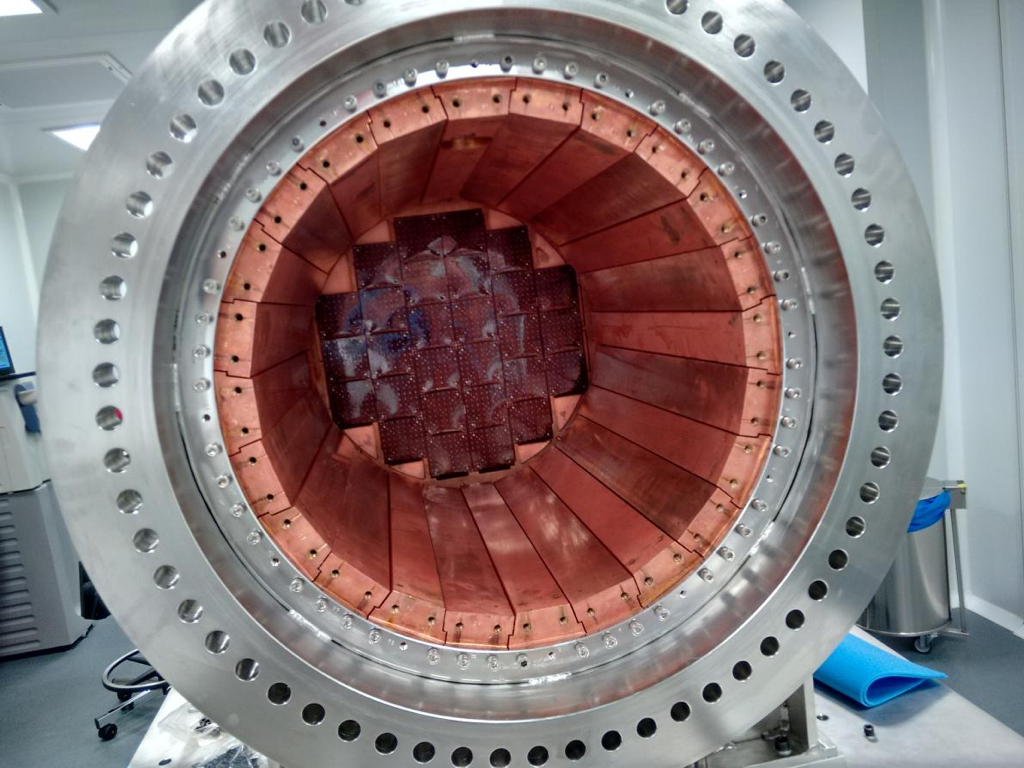
\includegraphics[height=8cm]{img2/TrackingPlaneFromEP.png}

\caption{The NEW tracking plane. Top: A drawing, showing the KDBs over-covering the fiducial area;.
Middle: The KDBs installed in the TP support plate. Bottom: The TP seen from the EP side.} \label{fig:NTP}
\end{figure}

The NEW tracking plane, shown in figure \ref{fig:NTP}, permits the reconstruction of the trajectories of charged particles (e.g., electrons) in the NEW/NEXT detectors. It consists of a matrix of silicon photomultipliers (SiPMs) which operate as light pixels, providing a 2D picture of the event (the third coordinate is given by the drift time). The SiPMs are radiopure 1-mm sensors, manufactured by SENSL. The TP is made of 28 radiopure circuits called Kapton DICE-Boards (KDBs). Each KDB has an $8\times8$~ SiPM array, where each SiPM is placed at a 1-cm pitch. Each KDB also includes a NTC temperature sensor and one LED for calibration. The KDBs over-cover the fiducial region with $\sim$1800 SiPMs, ensuring that there are no dead regions. The connector is located at the end of a long tail and is screened from the gas, in the fiducial volume, by a 120 mm thick copper shield.

%\subsubsection*{Silicon photomultipliers}\label{sec:sipms}
%A Silicon PhotoMultiplier (SiPM) consists of a matrix of photodiodes (diode which converts light into current), operating in Geiger mode. These photodiodes are connected in parallel becoming each one a pixel of the SiPM. A detailed picture of this structure is shown in figure~\ref{fig:sipm}. The pixels are connected by aluminum stripes to read out the combined signals, which is the sum of all pixels. The pixels are electrically decoupled by polysilicon resistive stripes between the pixels. 
%
%The SiPM used in the NEW detector are the SensL MicroFC-10035-SMT-GP model. This model has demonstrated to be sufficiently radiopure to operate in a low background experiment and also its dark current ($\sim100kHz/mm^2$) is much lower than in the previous models, allowing for easier calibration and an improved threshold for low energy events.
%
%
%\begin{figure}[hpt!]
%  \centering
%  \subfloat[\textit{Detail of the pixel array}]{%\label{fig:cabling:}
%  \includegraphics[height=0.22\textwidth]{TrackingPlane/IMG/PixelMatrix.pdf}}   
%  \hspace{5mm}             
%  \subfloat[\textit{Hamamatsu SiPM}]{%\label{fig:ad:ads7883}
%  \includegraphics[height=0.22\textwidth]{TrackingPlane/IMG/sipm.jpg}}
%  \hspace{5mm}             
%  \subfloat[\textit{SiPM from SensL}]{%\label{fig:ad:ads7883}
%  \includegraphics[height=0.22\textwidth]{TrackingPlane/IMG/sensl.jpg}}
%  \caption{\textit{Silicon photomultipliers}}
%  \label{fig:sipm}
%\end{figure}
%

\subsubsection*{KDB arrangement and cabling}
\label{sec:DB}

A scheme of the TP cabling is shown in 
figure \ref{fig:cabling:scheme}). The engineering problems that had to be solved were: a) to place connectors behind the copper shielding; b) to pass the KDB analog signals through custom feedthroughs; c) to transport the signals to the front-end electronics, via long-cables.  

\begin{figure}[hpt!]
    \bigskip
    \begin{center}\leavevmode
        \rotatebox{0}{
        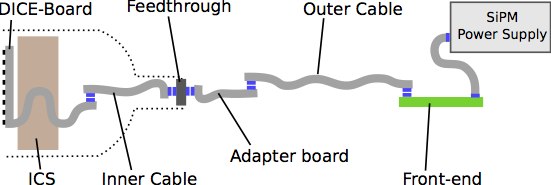
\includegraphics[width=.8\textwidth]{img2/Simple.png}}
        \caption{\textit{Tracking plane cabling scheme.}}
        \label{fig:cabling:scheme}
    \end{center}
\end{figure}



%Fig. \ref{fig:spring_detail} shows the detail of one of those springs.

%\begin{figure}[h!]
%\begin{center}
%\includegraphics[width=0.45\textwidth]{TrackingPlane/IMG/spring_plate_detail}
%%\hspace{15mm}
%%\includegraphics[width=0.39\textwidth]{IMG/DB.JPG}
%\caption{Detail of one of the springs in the tracking plane thin plate that will allow to accommodate the tracking plane perfectly parallel to the electroluminescence region.}
%\label{fig:spring_detail}
%\end{center}
%\end{figure}


\begin{figure}[hpt!]
\begin{center}
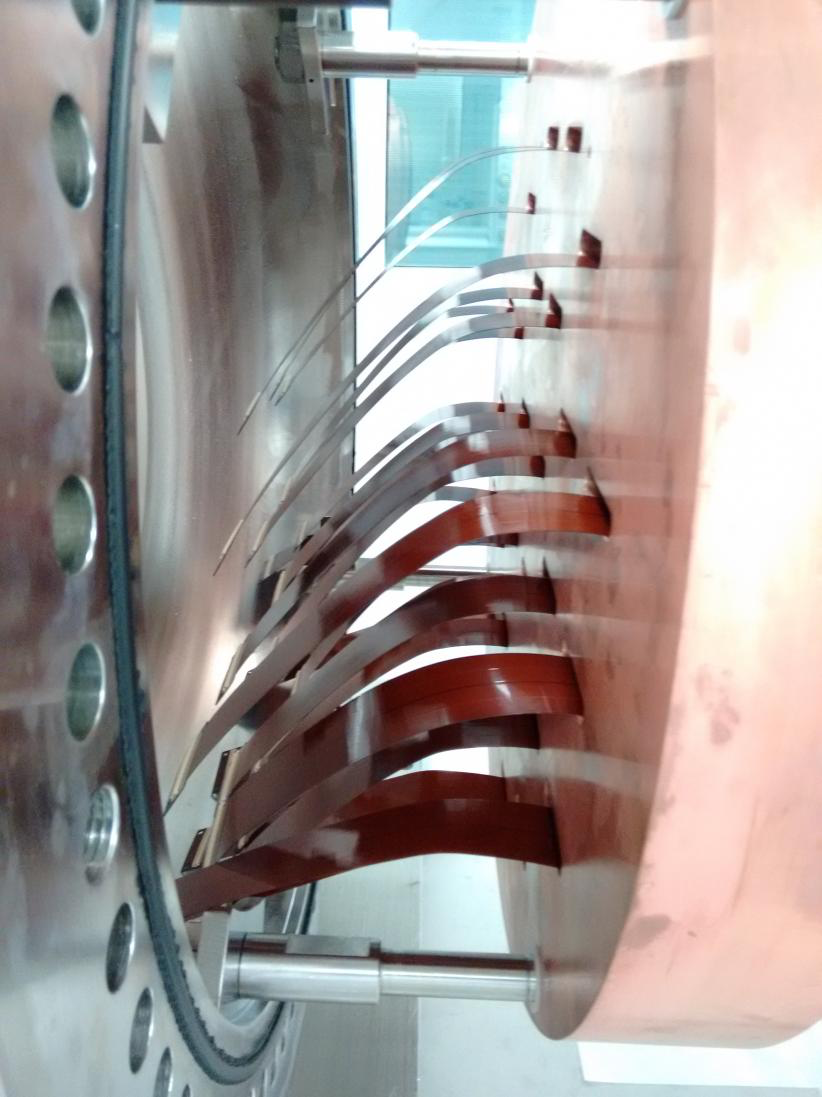
\includegraphics[width=8cm]{img2/cabling.png}
\caption{Dice-Boards cables passing through the holes in the shielding plate. At the end of the tail there is a connector that will allow for an extension of the cable to reach the feedthrough.}
\label{fig:cabling}
\end{center}
\end{figure}

\begin{figure}[hpt!]
\begin{center}
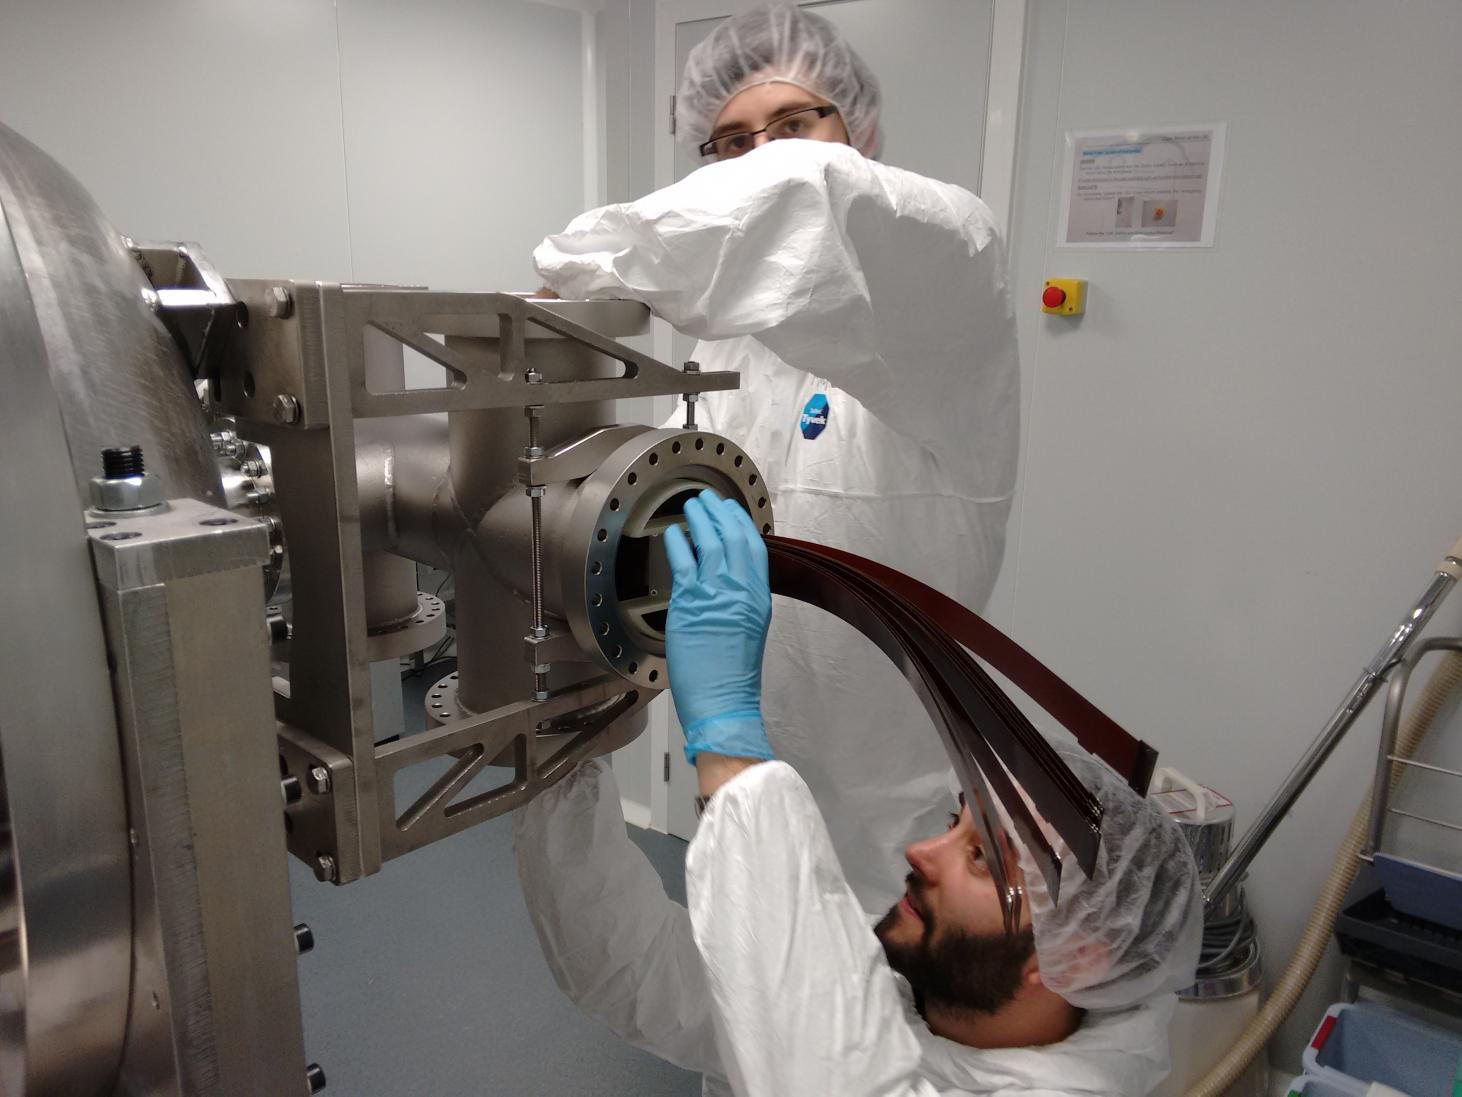
\includegraphics[width=12cm]{img2/cabling_spaceship.png}
%\includegraphics[width=0.45\textwidth]{TrackingPlane/IMG/spacechip_cabling}
%\includegraphics[width=0.45\textwidth]{TrackingPlane/IMG/spaceship_unmounted}
\caption{Cables being extracted from the ``spaceship'' during TP assembly, at the LSC clean room.}
\label{fig:cabling_spaceship}
\end{center}
\end{figure}

The KDBs were mounted on top of a thin plate of copper held by springs to the main copper plate which acts as a shield. The purpose of these springs is to allow for a small movement of the plate during the assembly and closing of the detector, allowing for a perfect match of the tracking plane with the EL region. 

Once the KDBs are mounted, the tail has to be passed through the holes in the shielding plate (figure \ref{fig:cabling_spaceship}). At the end of the tail a connector is soldered to connect a cable extension made of the same materials as the DICE-Boards. These cables have to be organised to reach 5 different feed-throughs. The distribution of the cables is done using 3D printed structures placed inside a steel structure that will allow for the extraction of the SiPM cables and also is the point at which the piping for vacuum and evacuation connects.


The final step in the connection of the inner cables of the tracking plane is the connexion to the tracking-plane feedthroughs (TPFT). Each one of these custom-made FTs allows up to 6 KDB connexions. Extracting the signals of the 29 KDBs therefore requires 5 TPFTs. Figure \ref{fig:TPFT} shows the front and the back side of the TPFT as well as the cable connexion.

\begin{figure}[hpt!]
\centering
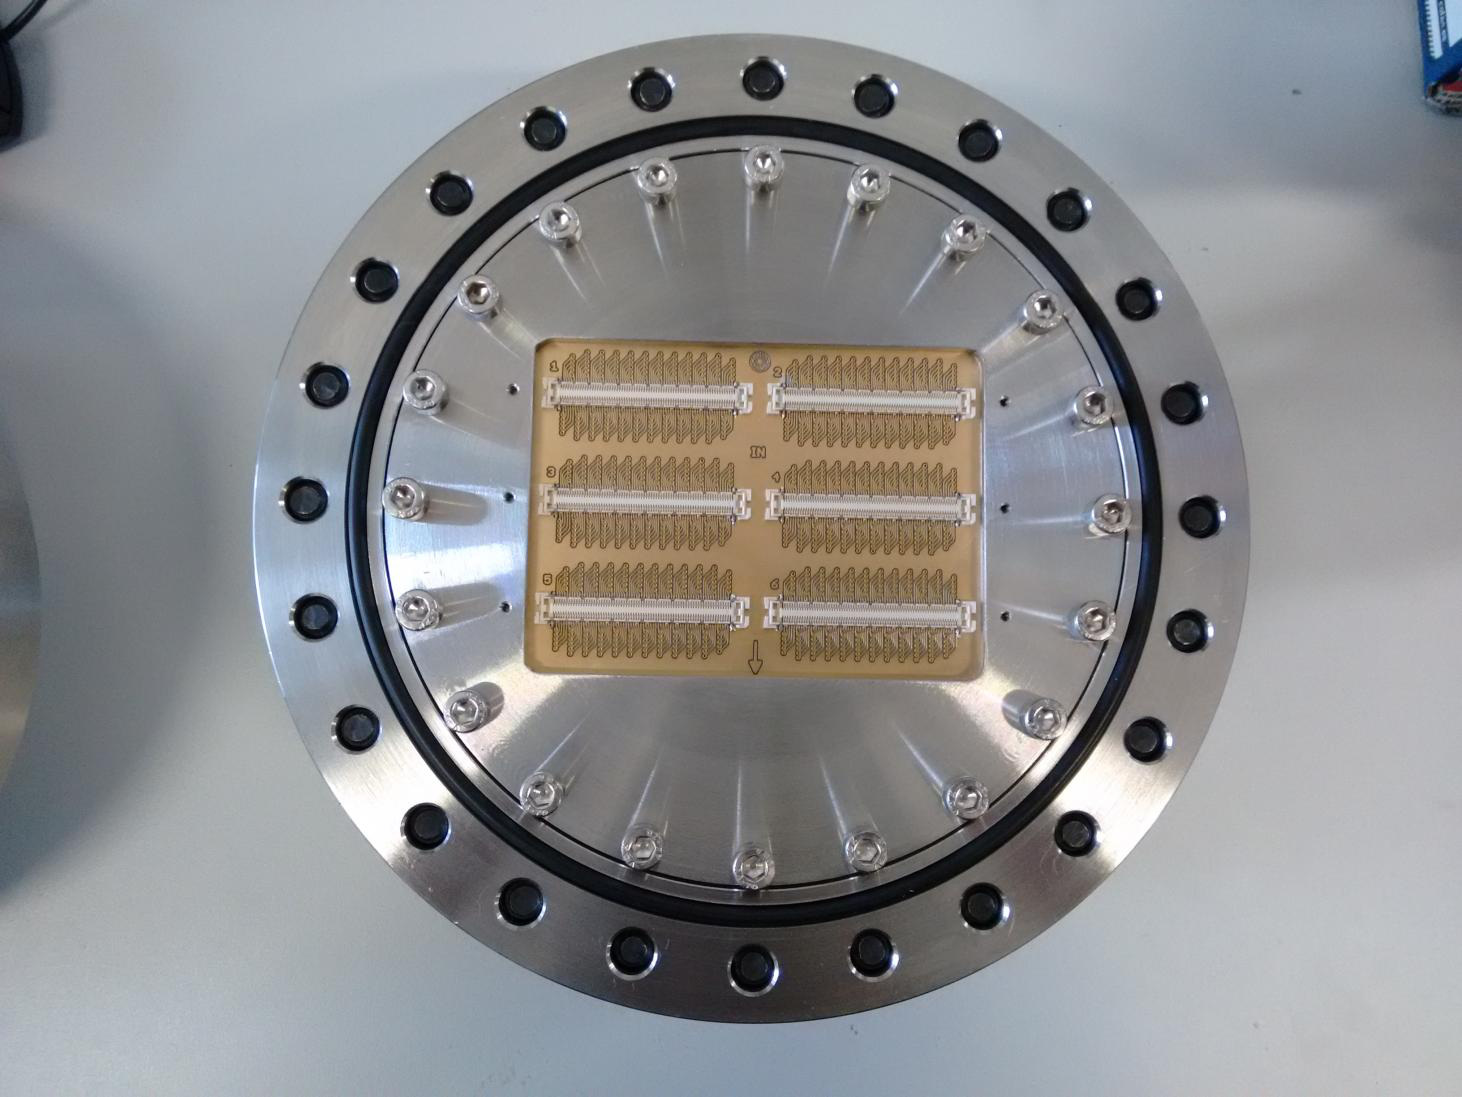
\includegraphics[width=0.45\textwidth]{img2/TPFT1.png}
%\includegraphics[width=0.45\textwidth]{TrackingPlane/IMG/TPFT2}
%\includegraphics[width=0.45\textwidth]{img/TPFTI.png}
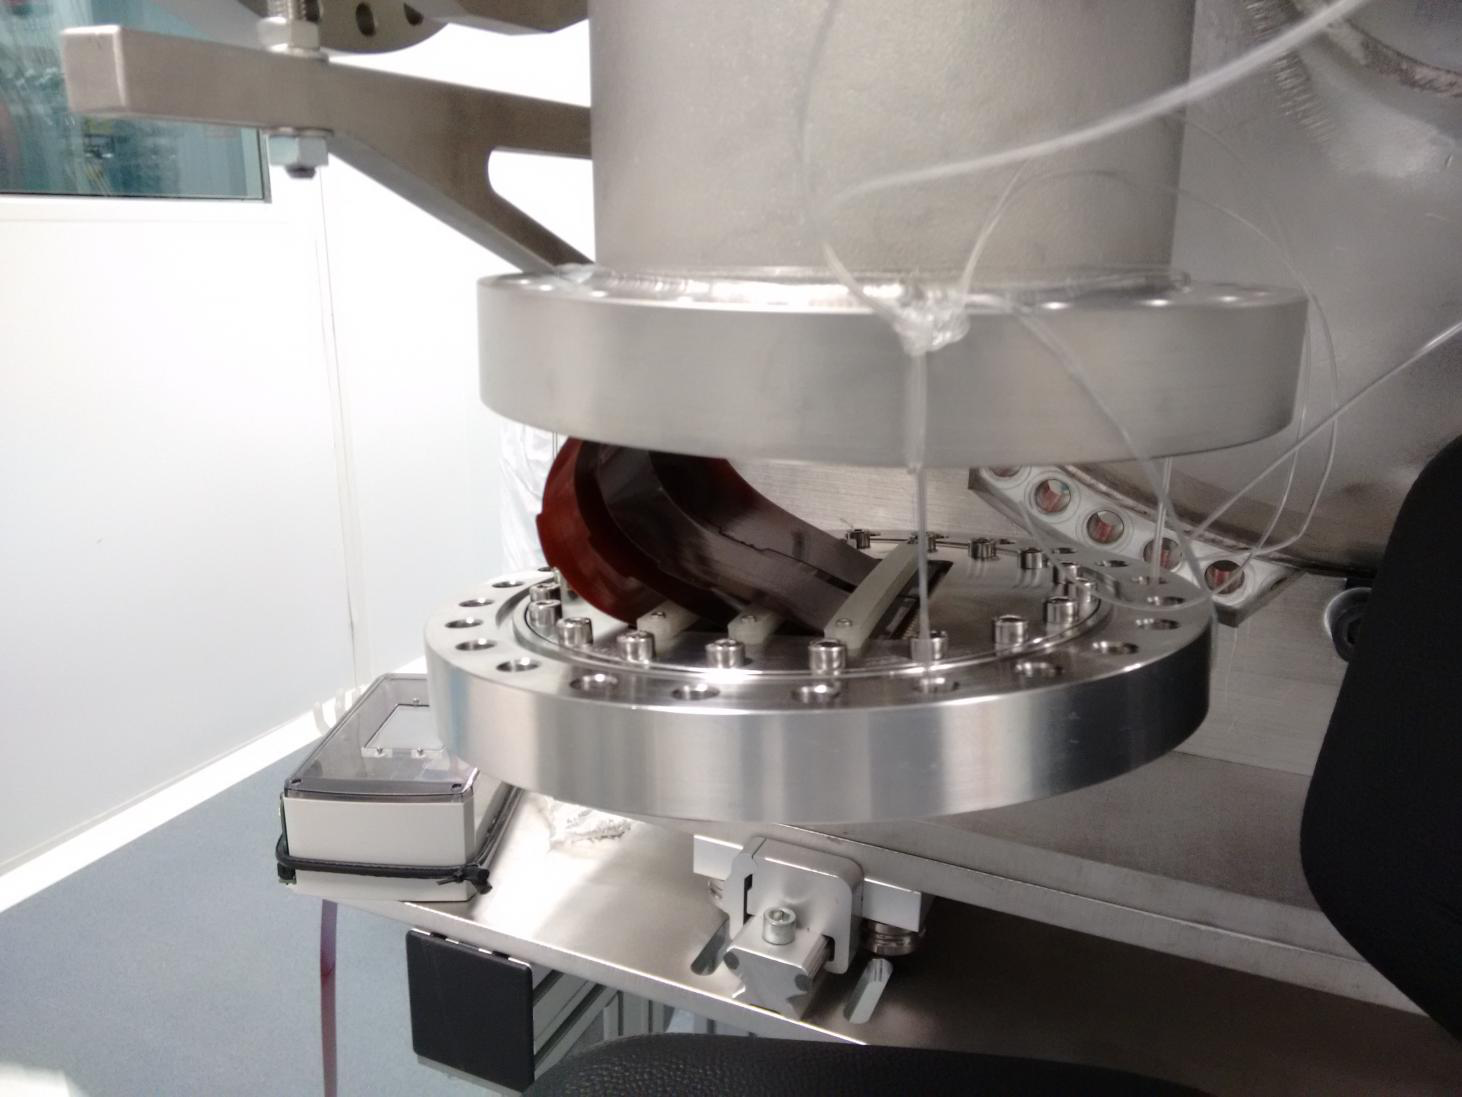
\includegraphics[width=0.45\textwidth]{img2/TPFT_connected.png}
\caption{The tracking-plane feedthroughs (TPFTs). Left: Inner side of the TPFT. Right: Cable connexion.}
\label{fig:TPFT}
\end{figure}


\subsubsection*{External cabling}\label{sec:ext}


\begin{figure}[hpt!]
\centering
\includegraphics[width=.45\textwidth]{img2/KrakenInLC.png}
\includegraphics[width=.45\textwidth]{img2/krakenOutOfLC.png}
%\includegraphics[width=.45\textwidth]{img2/cabling_under_platform.png}
\includegraphics[width=.45\textwidth]{img2/cabling_under_platform.png}
\includegraphics[width=.45\textwidth]{img2/cabling2FEE.png}
\caption{Different parts of the external cabling of the tracking plane. The image at the upper left shows the cables being directed to the exit hole of the lead castle. The upper right image shows the cables coming out of the lead castle. The bottom left image shows how the cables move under the platform. The bottom right image shows in detail the connexion of the cables to the FEE boards.}
\label{fig:external_installation}
\end{figure}

In order to keep background events to a minimum, front-end electronics are placed nearby the detector but beyond the lead castle that surrounds the TPC, with a total cable length of $\sim$ 5 m from the sensor to the electronics. This poses a challenge in the design of a cabling solution that (1) is radio-clean enough to be inside the detector, (2) keeps enough signal-to-noise ratio in the relevant signal bandwidth for the gated integrator with a 5 m cable, (3) is cost-effective, (4) includes SiPM biasing voltage wires and (5) is also valid for the final NEXT phase (NEXT-100).

Differential transmission lines on fine-pitch FFC cables outside the detector were chosen as a good trade-off between performance and cost. The cables are 0.5 mm pitch with $280 \times 76 \mu$m traces embedded in a thin polyester layer. The anode and the cathode of each SiPM are connected to the \textit{signal} and \textit{bias} lines respectively. Channels are separated by a guard trace connected to the analog ground in the front-end. Therefore three lines are needed for each SiPM channel. In addition, each KDB adds several more lines for the temperature sensor and  calibrating LEDs.

%\begin{figure}[hpt!]
%\centering
%\includegraphics[width=.6\textwidth]{TrackingPlane/IMG/section.pdf}
%\caption{Cross-section of the external cable (just two channels are shown).}
%\label{fig:external}
%\end{figure}

Since commercial cables with the required density of traces were not available, the adopted solution was to split into four FFC cables. This way, the signals of an entire DICE-Board are distributed in four cables of 51 wires each. This distribution is done just at the output of the feedthrough, using a Kapton adapter board. This board has the same stackup as the DICE-Board or the inner cable, and splits the signals in four \textit{DF9 Hirose} connectors for the long cables.

In order to further reduce the noise coupled to the external cables, they are wrapped with a 1 mm aperture mesh, also connected to the analog ground at the front-end. This mesh is has its maximum attenuation rated at 1 MHz, which covers the range of frequencies we want to attenuate.

The external cables cables have been connected to the output of the TPFT and are passed below the platform to the location of the FEE boards where they are connected, as shown in figure \ref{fig:external_installation}.

%\subsubsection*{Sensor characterisation}
%The simplest method to calibrate the SiPMs is shown in figure \ref{fig:calibration} (top panel), and consists  in finding the different peaks associated to the different photoelectron numbers in the SiPM and extract the gain according to their separation. The first results from NEW show that the gain spread among the SiPMs is very small (figure \ref{fig:calibration} bottom).
%%The first data extracted from the tracking plane has been used to make a first evaluation of the behaviour of the different sensors and DICE boards. The SiPMs have been tested with no light (only dark counts were recorded) and with light pulses from the blue LEDs installed in the energy plane (Fig. \ref{fig:calibration} bottom).
%
%\begin{figure}[hpt!]
%\centering
%\includegraphics[width=0.45\textwidth]{TrackingPlane/IMG/normal_calibration}
%\includegraphics[width=0.45\textwidth]{TrackingPlane/IMG/SIPMsGain}
%%\includegraphics[width=0.45\textwidth]{IMG/SiPM_LED_noLED}
%\caption{Top: standard method for calibration where the charge corresponding to the different number of photoelectrons in the SiPMs is estimated with a fit to the peak. The gain of the SiPM is calculated using the separation of the different peaks. Bottom: Histogram showing the gain of all the SiPMs in the plane. This histogram shows that the spread on the SiPMs gain is only of the order of a few ADC counts. 
%%Bottom: Comparison of two spectra from the same SiPM, with (blue) and without light (red).
%}
%\label{fig:calibration}
%\end{figure}

\subsubsection*{Reflectors}

The material of choice for the KDBs (Kapton) has many advantages including flexibility, little degassing and radiopurity. However it is a poor reflector. In order to increase the amount of light recorded by the energy plane, a 2 mm teflon reflector is placed in front of each KDB. The reflectors (figure \ref{fig:reflector}) have holes to accommodate the SiPMs without damaging them and also have a space for the thermal sensor and the LEDs. However no holes are necessary for the LEDs, since teflon is sufficiently transparent to the blue light they emit. 
\begin{figure}[hpt!]
\centering
%\includegraphics[width=0.45\textwidth]{TrackingPlane/IMG/teflon1}
\includegraphics[width=0.45\textwidth]{img2/teflon2.png}
\includegraphics[width=0.45\textwidth]{img2/HalfAndHalf.png}

\caption{Top: Front side (EL) of the reflector. Bottom: The TP, half-covered with the reflectors.}
\label{fig:reflector}
\end{figure}

%\subsection{The front-end electronics and DAQ} 
%
%%%%%%%%%%%
%\begin{figure}
%\centering
%\includegraphics[width=0.7\paperwidth]{img/FEE_SiPM.pdf}
%\caption{\small Functional blocks in the FEB card.}
%\label{fig:feb}
%\end{figure}
%
%The front-end electronics for the PMTs in NEW and NEXT-100 will be very similar to the system developed for the NEXT-DEMO prototype. The first step in the chain is to shape and filter the fast signals produced by the PMTs to match the digitiser and eliminate the high frequency noise. An integrator is implemented by simply adding a capacitor and a resistor to the PMT base. The charge integration capacitor shunting the anode stretches the pulse and reduces the primary signal peak voltage accordingly.
%
%The electronics for the SiPMs is very simple. Our design consists of a  64 channel Front-End Board (FEB, Figure~\ref{fig:feb}). Each FEB takes the input of a single DB (transmitted via low-crosstalk kapton flat cables) and includes the analog stages, ADC converters, voltage regulators and an FPGA that handles, formats, buffers and transmits data to the  DAQ. 
%
%The NEW and NEXT-100 data-acquisition systems (DAQ) follow a modular architecture named the Scalable Readout System (SRS), already described in our CDR \cite{Alvarez:2011my}. At the top of the hierarchy, a PC farm running the DAQ software, DATE, receives event data from the DAQ modules via Gigabit Ethernet (GbE) links. The DATE PCs (Local Data Concentrators, LDCs) assemble incoming fragments into sub-events, which are sent to one or more additional PCs (Global Data Concentrators, GDC). The GDCs build complete events and store them to disk for offline analysis.
%
%The DAQ modules used are Front-End Concentrator (FEC) cards, which serve as the generic interface between the DAQ system and application-specific front-end modules. The FEC module can interface different kinds of front-end electronics by using the appropriate plug-in card. The FEC card and the overall SRS concept have been developed within the framework of the CERN RD-51 collaboration. 

\subsection{Field Cage}

%\begin{figure}[hpt!]
%\centering
%\includegraphics[height=8cm]{img/NFC.pdf}
%\caption{The NEW field cage (NFC).} \label{fig:NFC}
%\end{figure}

\begin{figure}[hpt!]
\centering
\includegraphics[height=8cm]{img2/FieldCageWithRing.png}
\caption{Detail of the copper rings in the drift region.} \label{fig:drift1}
\end{figure}

The goal of the FC is to provide a homogeneous and uniform electric field inside the active volume of the NEW detector. The field cage has an outer diameter (OD) of 50 cm and a length of 50 cm. Thus, both the longitudinal and radial dimensions are roughly half of those of NEXT-100. 

The main body of the field cage is a high-density polyethylene (HDPE) cylindrical shell that provides electric insulation from the vessel. The shell is 2.5 cm thick. Two wire meshes (cathode and anode) define the active volume of NEW. The electroluminescence region is defined by one of these meshes (anode) and a fused silica plate (gate) with an ITO coating to make its surface resistive. Ultra pure copper strips attached to the HDPE and connected with low-background 
10G$\Omega$~ resistors (figure \ref{fig:drift1}) grade the high voltage to provide a homogeneous and uniform moderate electric field (300-600 V/cm) inside the active volume of the NEW detector.


\begin{figure}[hpt!]
\centering
\includegraphics[width=\textwidth]{img2/HVFT_full_image.png}
\includegraphics[width=\textwidth]{img2/HVFT_with_drift.png}
\caption{Design (top) and Comsol simulation (bottom) of the NEW HVFT.} \label{fig:hvft1}
\end{figure}


\begin{figure}[hpt!]
\centering
%\includegraphics[width=0.45\textwidth]{FieldCage/img/HVFT_tip_detail.jpg}
\includegraphics[width=0.75\textwidth]{img2/HVFT2.png}
\caption{A picture of the HVFT.} \label{fig:hvft_tip}
\end{figure}

%\begin{figure}[hpt!]
%\centering
%\caption{Detail of the HVFT tip. The copper conector has been designed  to minimise the electric field in the surface of the tip.} \label{fig:hvft_tip}
%\end{figure}

The most challenging parts of the field cage are the high voltage feedthroughs. These are penetrators which must be capable of holding very high voltages (up to 50 kV for the cathode penetrator and up to 20 kV for the anode) while at the same time being radiopure and gas-tight. Figure \ref{fig:hvft1} shows the design of the NEW HVFT. Figure 
\ref{fig:hvft_tip} shows a picture of the cathode HVFT. The initial tests show that the HVFT can hold a voltage in excess of 30 kV with only a few sparks per day. Work is in progress to reduce the number of sparks and increase the maximum voltage. However, 30 kV is sufficient for the initial period of commissioning at 10 bar with a drift field of 15 kV (300 V/cm over 50 cm) and en EL voltage of 15 kV. (E/P $\sim$~3). For NEXT-100 the HVFT needs to withstand 45-55 kV (depending on pressure and EL). Operation with NEW will be essential to improving the performance of the HVFT. 

The cathode grid consist of a stainless steel frame with wires to fix the potential (figure \ref{fig:cath}). It has
been built by Texas A\&M University and is currently at the LSC, ready to be installed (first week of May, 2016).

\begin{figure}[hpt!]
\centering
\includegraphics[width=0.45\textwidth]{img2/cathode_1.png}
\includegraphics[width=0.45\textwidth]{img2/cathode_tensioners.png}
\caption{Cathode frame (left), showing in detail the grooves for fixing the wires. The bronze tensioners (right) will be used to adjust every wire to the appropriate tension.} \label{fig:cath}
\end{figure}

\begin{figure}[hpt!]
\centering
%\includegraphics[width=0.45\textwidth]{FieldCage/img/mesh_grid_1.jpg}
\includegraphics[width=0.45\textwidth]{img2/SS_grids_1.png}
\includegraphics[width=0.45\textwidth]{img2/Anode_coated.png}
\caption{(Left) The frames used for assembling and tightening the gate mesh. (Right)  A picture of the fused silica plate before coating with ITO.} \label{fig:el}
\end{figure}

The electroluminescent region (EL) is the amplification region of the detector (figure \ref{fig:el}).  The main parts of the EL region are the mesh and the anode. The anode consists of a plate of fused silica coated with ITO on one side and TPB on the other. The fused silica with the ITO layer was produced by Texas A\&M and arrived at the end of May 2015. It was coated at the LNGS coating facilities and is ready for installation. The gate mesh is also ready for installation.




%Due to the intensity of the electric field sparks may occur while operating the detector but they will happen inside the detector and so they do not represent a safety issue.

%When installing the detector the fused silica plate needs to be treated very carefull. Only people authorized by the experiment may be allow to do that.






%\section{The NEW project}
% \label{sec.nproj}
%
%\begin{figure}
%\centering
%\includegraphics[width=0.7\paperwidth]{img/NEWProject.pdf}
%\caption{\small The NEW project.}
%\label{fig:NEWProject}
%\end{figure}
%
%The NEW project is organised in terms of sub-projects, called NEW projects or NPR. They are:
%\begin{enumerate}
%\item {\bf Infrastructures}: Construction and commissioning of the mechanical infrastructures (platform, pedestal and lead castle). The project leader is 
%Jose Luis P\'erez (UPV).
%\item {\bf Gas system}: Construction and commissioning of the NEW gas system. The project leader is 
%Igor Liubarsky (IFIC).
%\item {\bf Pressure Vessel}: Construction and commissioning of the NPV, the support table and the opening--closing system. Interfaces with the NFC, NEP and NTP projects. The project leader is 
%Sara C\'arcel (IFIC).
%\item {\bf Field Cage}: Design, construction and commissioning of the NFC, HVFT and EL grids. The project leader is Clement Softka (Texas A\&M). Interfaces with NPV, NEP and NTP.
%\item {\bf Energy plane}: Design, construction and commissioning of the NEP. Interfaces with NFC and NPV. The project leader is 
%Andrew Laing (IFIC).
%\item {\bf Tracking plane}: Design, construction and commissioning of the NTP. Interfaces with NFC and NPV. The project leader is 
%Francesc Monrabal (IFIC).
%\item {\bf FEE}: Design, fabrication and commissioning of the front-end electronics for the PMTs and the SiPMs. Interfaces with NEP and NTP. The project leader is 
%Francisco Toledo (UPV).
%\item {\bf DAQ}: Design, fabrication and commissioning of the data acquisition modules for NEW. Interfaces with FEE. The project leader is 
%Raul Esteve (UPV).
%\item {\bf Slow control}: Design, fabrication and commissioning of the slow control for NEW. Interfaces with all systems that must be controlled. The project leader is 
%Javier Rodr\'iguez (IFIC).
%\item {\bf Online}: Design and commissioning of the online monitoring for NEW. Interfaces with offline, DAQ and Slow Control. The project leader is 
%Toni Mar\'i (UPV).
%\item {\bf Offline}: Design and commissioning of the offline for NEW. Interfaces with online, DAQ and Slow Control. The project leader is 
%Justo Mart\'in-Albo (IFIC).
%\item {\bf Calibration}: Design and commissioning of the calibration systems and procedures for NEW. Interfaces with pressure vessel, field cage and offline. The project leader is 
%Paola Ferrario (IFIC).
%\item {\bf Integration}: Coordinates the integration of the full system at the LSC. The project leader is 
%Teopisti Dafni (UNIZAR).
%\item {\bf Radiopurity}: Coordinates the screening of all the components of NEW and keeps the NEXT background model data base. The project leader is 
%Susana Cebri\'an (UNIZAR).
%\end{enumerate}
%
%
%Figure \ref{fig:NEWProject} shows a summary cronogram of the NEW project. A full resource-load project is being prepared by the technical coordinator (IL) and the spokesperson. The current program allows the construction of NEW and the completion of the needed infrastructures by early 2015. A commissioning period of 6 months is foreseen, followed by at least 12 months of run with enriched xenon. 



\section{Conclusions}
\label{sec.conclu}

A progress report of the NEXT project has been presented. The report describes the progress in the construction and commissioning of the experiment infrastructure and the NEW detector during 2015 and the first quarter of 2016. In summary:

\begin{itemize}
\item The working platform, seismic pedestal and lead castle are completed and operational.
\item The full NEXT gas system, including recirculation, purification, emergency storage and cryo-recovery is ready to be certified for operation (scheduled for May, 2016).
\item The NEW detector is being assembled at the LSC. The energy plane and tracking plane are already installed and the field cage is scheduled for installation in May, 2016.
\item The collaboration is completing the risk assessment needed for regular operation at the LSC. 
\item The Slow Controls are ready to operate. 
\item The plan for the second semester of 2016 is to commission the detector, identifying technical issues and ensuring the stability and reliability of the apparatus and gas system. 
\item The set of measurements foreseen for the initial operation period include the measurement of the electron lifetime, and calibrations with LEDs and radioactive sources. 
\item The calibration aims at producing a first measurement of the NEW energy resolution by the November, 2016, LSCSC meeting. 
\end{itemize}




\bibliographystyle{JHEP}
\bibliography{references}

\end{document}
%%%